\documentclass[11pt,reqno]{amsart}

\usepackage[utf8]{inputenc}
\usepackage[T1]{fontenc}
\usepackage{lmodern}
\usepackage{amsmath,amssymb,amsfonts,amsthm,mathtools}
\usepackage{booktabs,array,multirow}
\usepackage{graphicx}
\usepackage{enumitem}
\usepackage[margin=1.0in]{geometry}
\usepackage{microtype}
\usepackage{xcolor}
\definecolor{linkblue}{rgb}{0.0,0.2,0.6}
\usepackage[colorlinks=true,linkcolor=linkblue,citecolor=linkblue,urlcolor=linkblue]{hyperref}

\newtheorem{theorem}{Theorem}[section]
\newtheorem{proposition}[theorem]{Proposition}
\newtheorem{lemma}[theorem]{Lemma}
\newtheorem{corollary}[theorem]{Corollary}
\theoremstyle{definition}
\newtheorem{definition}[theorem]{Definition}
\theoremstyle{remark}
\newtheorem{remark}[theorem]{Remark}

\numberwithin{equation}{section}
\allowdisplaybreaks

\newcommand{\R}{\mathbb{R}}
\newcommand{\C}{\mathbb{C}}
\newcommand{\N}{\mathbb{N}}
\newcommand{\Z}{\mathbb{Z}}
\newcommand{\dd}{\mathrm{d}}
\newcommand{\ee}{\mathrm{e}}
\newcommand{\ii}{\mathrm{i}}
\newcommand{\Rea}{\mathrm{Re}}
\newcommand{\Ima}{\mathrm{Im}}
\newcommand{\sinch}{\mathrm{sinc}_{\mathrm{hyp}}}
\newcommand{\fac}{\mathclose{\mathchar"0021}}

\title[Second-Order De~Branges--Nevanlinna Kernels and Blind Spots]{Second-Order De~Branges--Nevanlinna Kernels, Derivative-Wronskian Splitting, Davenport--Heilbronn Blind Spots, and the Differential Threshold $\beta^*$}

\author{Thijs Missiaen}
\address{Independent Researcher, Belgium}
\email{thijs.missiaen@gmail.com}
\thanks{ORCID: \href{https://orcid.org/0009-0007-3678-0810}{0009-0007-3678-0810}}

\subjclass[2020]{Primary 11M06, 11M26; Secondary 30D15, 46E22}
\keywords{Riemann $\Xi$-function, transverse Wronskian, de~Branges--Nevanlinna kernel, Davenport--Heilbronn function, Jensen differential operators, Lehmer pairs, Wigner phase-space distribution, de~Bruijn--Newman constant}
\dedicatory{\upshape November 2026}
\date{November 2026}

\begin{document}
\sloppy

\begin{abstract}
For a real-entire function $F(z)$ and couplings $\alpha, \beta > 0$, we study the second-order structure function $E_{\alpha,\beta}(z) := F(z) - \ii\alpha F'(z) - \beta F''(z)$ and its de~Branges--Nevanlinna kernel $K_{\alpha,\beta}(z_1, z_2)$. On the diagonal $w = t - \ii d$, all three squared moduli and $-2\beta\Rea(\overline{F}F'')$ cancel identically, giving $K_{\alpha,\beta}(w,w) \equiv \frac{\alpha}{\pi}\widetilde{W}_{0,1}(d,t) + \frac{\alpha\beta}{\pi}\widetilde{W}_{1,2}(d,t)$. For Riemann's $\Xi$-function, this lifts the $d=0$ Lehmer near-coalescence degeneracy at order $d^0$, couples $\widetilde{W}_{1,2}$ to $\widetilde{W}_{0,1}$ via a radial four-dimensional Laplace operator, and extends to order-$M$ Hurwitz chains. Crucially, however, Hermite--Biehler positivity of $E_{\alpha,\beta}$ for fixed $\beta > 0$ corresponds only to real zeros of $F - \beta F''$, strictly weaker than real zeros of $F$. Evaluating $K_{\alpha,\beta}^{\mathrm{DH}}$ on the Davenport--Heilbronn function exposes an explicit blind spot: at its critical-line defect $\tau_{\mathrm{false}} \approx 85.7472$, $\pi K_{1,\beta}^{\mathrm{DH}} > 0$ for all $\beta > 0.053495$, motivating the open differential threshold $\beta^*(F) := \inf\{\beta \in \R : F - \beta F'' \text{ has only real zeros}\}$.
\end{abstract}

\maketitle

\section{Introduction and main results}\label{sec:intro}

In the analytic theory of Hilbert spaces of entire functions~\cite{debranges1968,debranges1986,debranges1992} associated with Riemann's completed zeta function $\Xi(z) := \xi(\frac{1}{2} + \ii z)$ ($z = t - \ii d$, $s = \frac{1}{2} + d + \ii t$)~\cite{riemann1859,polya1926,titchmarsh1986}, linear and higher-order differential combinations of $\Xi(z)$ provide natural test families for Hermite--Biehler positivity~\cite{jensen1913,lagarias1999,lagarias2006}. While Conrey and Li~\cite{conreyli2000} proved that global inner-product positivity conditions on classical Sonine--de~Branges spaces fail for $\xi(s)$, Lagarias~\cite{lagarias1999,lagarias2006} studied the first-order structure function $E_\alpha(z) := \Xi(z) - \ii\alpha\,\Xi'(z)$ ($\alpha > 0$), whose diagonal de~Branges--Nevanlinna kernel reduces to the parity-reduced transverse Wronskian
\begin{equation}\label{eq:intro_first_order}
K_\alpha(t - \ii d,\, t - \ii d) := \frac{|E_\alpha(t - \ii d)|^2 - |E_\alpha^\#(t - \ii d)|^2}{4\pi d} \equiv \frac{\alpha}{\pi}\,\widetilde{W}_{0,1}(d,t),
\end{equation}
where $W_{0,1}(d,t) := \frac{1}{2}\partial_d|\Xi(t-\ii d)|^2$ and $\widetilde{W}_{0,1}(d,t) := d^{-1}W_{0,1}(d,t)$~\cite{speiser1934,hinkkanen1997,csordas1986,griffin2019}. By Hinkkanen's monotonicity criterion~\cite{hinkkanen1997} and Lagarias's positivity theorem~\cite{lagarias1999}, $E_\alpha$ belongs to the Hermite--Biehler class with respect to $\C_- = \{t - \ii d : d > 0\}$ if and only if the Riemann Hypothesis holds.

On the critical line $d = 0$ itself, however, the first-order kernel~\eqref{eq:intro_first_order} exhibits a local near-coalescence degeneracy whenever two simple zeros approach a Lehmer pair~\cite{lehmer1956}: at a hypothetical double zero $t_0 \in \R$ ($\Xi(t_0) = \Xi'(t_0) = 0$, $\Xi''(t_0) \neq 0$), the critical-line Laguerre invariant $\pi K_\alpha(t_0, t_0) = \alpha((\Xi'(t_0))^2 - \Xi(t_0)\Xi''(t_0)) = \alpha c_1(t_0) = 0$ vanishes at order $d^0$, so positivity appears only transversely at order $d^2$ via $c_3(t_0) = \frac{1}{2}(\Xi''(t_0))^2 > 0$. Equivalently, at the local extremum $t_{\mathrm{mid}}$ ($\Xi'(t_{\mathrm{mid}}) = 0$) between a closely spaced Lehmer pair $t_\pm = t_{\mathrm{mid}} \pm \delta$ ($\delta \to 0$), $\pi K_\alpha(t_{\mathrm{mid}}, t_{\mathrm{mid}}) = -\alpha\Xi(t_{\mathrm{mid}})\Xi''(t_{\mathrm{mid}}) = \mathcal{O}(\delta^2) \to 0$.

A natural question is what happens both algebraically and zero-theoretically when one passes from $E_\alpha(z)$ to the second-order differential structure function
\begin{equation}\label{eq:intro_E_alpha_beta}
E_{\alpha,\beta}(z) := F(z) - \ii\alpha\,F'(z) - \beta\,F''(z) \qquad (\alpha > 0,\; \beta > 0),
\end{equation}
including the repeated-root operator $(1 - \frac{\ii\alpha}{2}\partial_z)^2 F(z)$ ($\beta = \alpha^2/4$). In this paper we give a complete two-sided answer. On the algebraic side, we prove that $K_{\alpha,\beta}$ splits without cross-term contamination into $\frac{\alpha}{\pi}\widetilde{W}_{0,1} + \frac{\alpha\beta}{\pi}\widetilde{W}_{1,2}$, lifts the $d=0$ Lehmer near-coalescence degeneracy at order $d^0$, and satisfies a radial four-dimensional Laplace PDE and dipole recursion. On the zero-theoretic side, we prove that \emph{unlike} $E_\alpha(z)$, Hermite--Biehler membership of $E_{\alpha,\beta}(z)$ for fixed $\beta > 0$ does \emph{not} imply that $F(z)$ has only real zeros: it corresponds only to real zeros of $A_\beta(z) := F(z) - \beta F''(z)$ interlacing with $F'(z)$~\cite{debranges1968,jensen1913,polya1927}. Evaluating $K_{\alpha,\beta}$ on the self-dual Davenport--Heilbronn function~\cite{davenportheilbronn1936} demonstrates that for $\beta > 0.053495$ (including $\beta = \frac{1}{4}$), the positive second-order term $+\beta\widetilde{W}_{1,2}$ overwhelms the negative Laguerre defect $c_1^{\mathrm{DH}}(\tau_{\mathrm{false}}) < 0$ and renders $K_{\alpha,\beta}^{\mathrm{DH}}$ blind to actual off-line zeros.

\begin{theorem}[Main Structural and Blind-Spot Results]\label{thm:main}
Let $F(z)$ be a real-entire function ($\overline{F(\bar{z})} = F(z)$), let $z = t - \ii d \in \C$ with $d \in \R \setminus \{0\}$ and $t \in \R$, and set $E_{\alpha,\beta}(z) := F(z) - \ii\alpha F'(z) - \beta F''(z)$ and $E_{\alpha,\beta}^\#(z) := \overline{E_{\alpha,\beta}(\bar{z})} = F(z) + \ii\alpha F'(z) - \beta F''(z)$ for $\alpha, \beta \in \R$. Then:
\begin{enumerate}[label=\textup{(\roman*)},leftmargin=2.2em]
\item \textbf{Cross-Term-Free Kernel Splitting and Cauchy--Pick Decomposition.} In $|E_{\alpha,\beta}(t-\ii d)|^2 - |E_{\alpha,\beta}^\#(t-\ii d)|^2$, all three squared moduli $|F|^2, \alpha^2|F'|^2, \beta^2|F''|^2$ and the non-adjacent cross-term $-2\beta\Rea(\overline{F}F'')$ cancel identically, yielding
\begin{equation}\label{eq:intro_second_order_split}
K_{\alpha,\beta}(t - \ii d,\, t - \ii d) := \frac{|E_{\alpha,\beta}(t - \ii d)|^2 - |E_{\alpha,\beta}^\#(t - \ii d)|^2}{4\pi d} \equiv \frac{\alpha}{\pi}\,\widetilde{W}_{0,1}(d,t) + \frac{\alpha\beta}{\pi}\,\widetilde{W}_{1,2}(d,t),
\end{equation}
where $\widetilde{W}_{k,k+1}(d,t) := \frac{1}{2d}\partial_d|F^{(k)}(t-\ii d)|^2$ ($k = 0, 1$). For any nodes $z_1, \dots, z_M \in \C_-$, the $M \times M$ Cauchy--Pick matrix $[\mathbf{G}_{\alpha,\beta}]_{j,k} = K_{\alpha,\beta}(z_j, z_k)$ splits as $\mathbf{G}_{\alpha,\beta} \equiv \alpha\mathbf{G}^{(0,1)} + \alpha\beta\mathbf{G}^{(1,2)}$.
\item \textbf{Critical-Line Lehmer Lifting at Order $d^0$ and Square Interlocking for $\Xi$.} Specializing to $F = \Xi$ and $\alpha, \beta > 0$, taking $d \to 0^+$ yields $\pi K_{\alpha,\beta}(t,t) \equiv \alpha c_1(t) + \alpha\beta c_1^{(1)}(t)$ with $c_1 = (\Xi')^2 - \Xi\Xi''$ and $c_1^{(1)} = (\Xi'')^2 - \Xi'\Xi'''$. At the local extremum $t_{\mathrm{mid}}$ ($\Xi'(t_{\mathrm{mid}}) = 0$) between a simple Lehmer pair $t_\pm = t_{\mathrm{mid}} \pm \delta$, $-\Xi'(t_{\mathrm{mid}})\Xi'''(t_{\mathrm{mid}}) = 0$ vanishes identically, leaving $\pi K_{\alpha,\beta}(t_{\mathrm{mid}}, t_{\mathrm{mid}}) = -\alpha\Xi(t_{\mathrm{mid}})\Xi''(t_{\mathrm{mid}}) + \alpha\beta(\Xi''(t_{\mathrm{mid}}))^2 \ge \alpha\beta(\Xi''(t_{\mathrm{mid}}))^2 > 0$.
\item \textbf{Radial 4D-Laplace Coupling, Canonical Wigner Operator, and Hurwitz Chains.} The derivative Wronskian satisfies $\widetilde{W}_{1,2} \equiv \frac{1}{4}(\partial_d^2 + \frac{2}{d}\partial_d + \partial_t^2)\widetilde{W}_{0,1}$ and $c_{2m-1}^{(1)}(t) \equiv \frac{1}{4}(2m(2m+1)c_{2m+1}(t) + c_{2m-1}''(t))$ ($m \ge 1$). In canonical Wigner coordinates, $W_{1,2}(d,t) = 16\int_0^\infty y\sinh(2dy)\,I^{(1)}(y,t)\,\dd y$ with $I^{(1)}(y,t) = (y^2 + \frac{1}{4}\partial_t^2)I(y,t)$, giving Riemann--Siegel diagonal $\mathcal{D}_{1,2}(0,t) \sim \frac{1}{40}(\ln\frac{t}{2\pi})^5$ and horizon pair amplitude $|C_{N-1,N}^{(1,2)}| = \mathcal{O}(N(t)^{-5}) = \mathcal{O}(t^{-5/2})$. For any degree-$M$ Hurwitz polynomial $P_M(X) = \sum_{r=0}^M \alpha_r X^r$ ($\alpha_0 = 1, \alpha_r > 0$), $E_{\boldsymbol{\alpha}}(z) := P_M(-\ii\partial_z)\Xi(z)$ satisfies $\pi K_{\boldsymbol{\alpha}}(t_0, t_0) = +\alpha_{m-1}\alpha_m(\Xi^{(m)}(t_0))^2 + \mathcal{O}(\alpha_{>m})$ at a multiplicity-$m$ zero ($1 \le m \le M$).
\item \textbf{Davenport--Heilbronn Blind Spot and Zero Coalescence.} For the self-dual Davenport--Heilbronn function $\Xi_{\mathrm{DH}}(z)$, which has an off-line zero at $z_* \approx 85.699348 - 0.308517\ii$ and a critical-line Laguerre defect $c_1^{\mathrm{DH}}(\tau_{\mathrm{false}}) < 0$ at $\tau_{\mathrm{false}} \approx 85.747201$, the second-order kernel satisfies $\pi K_{1,\beta}^{\mathrm{DH}}(\tau_{\mathrm{false}}, \tau_{\mathrm{false}}) > 0$ for all $\beta > \beta_{\mathrm{blind}}^{(1)}(\tau_{\mathrm{false}}) \approx 0.05349534$ and $\pi K_{1,\beta}^{\mathrm{DH}}(z_*, z_*) > 0$ for all $\beta > 0$. Locally, the first conjugate zero pair of $\Xi_{\mathrm{DH}}(z) - \beta\Xi_{\mathrm{DH}}''(z)$ coalesces onto $\R$ at $\beta_{\mathrm{coal}}^{(1)} \approx 0.04467500$, whereas globally $\beta^*(\Xi_{\mathrm{DH}}) = +\infty$ because $\Xi_{\mathrm{DH}} - \beta\Xi_{\mathrm{DH}}''$ retains infinitely many zeros in $\sigma > 1$ for every fixed $\beta \in \R$.
\end{enumerate}
\end{theorem}

Representative $60$-decimal benchmark constants from Theorem~\ref{thm:main} (for $\alpha = 1, \beta = \frac{1}{4}$) are
\begin{equation}\label{eq:canonical_constants}
\begin{aligned}
K_{1,1/4}(\gamma_1, \gamma_1) &= 6.905897 \times 10^{-7}, & c_1^{(1)}(\tau_2) &= \bigl(\Xi''(\tau_2)\bigr)^2 = 6.741923 \times 10^{-11}, \\
\beta_{\mathrm{coal}}^{(1)}(\Xi_{\mathrm{DH}}) &= 0.0446750013, & \beta_{\mathrm{blind}}^{(1)}(\tau_{\mathrm{false}}) &= 0.0534953385, \\
\pi K_{1,1/4}^{\mathrm{DH}}(\tau_{\mathrm{false}}, \tau_{\mathrm{false}}) &= +2.378177 \times 10^{-56}, & \frac{|C_{N-1,N}^{(1,2)}(10^8)|}{\mathcal{D}_{1,2}(10^8)} &= 9.4585 \times 10^{-23}.
\end{aligned}
\end{equation}

\subsection{Proof overview}\label{subsec:proof_overview}

Our analysis combines four components across Sections~\ref{sec:kernel_split}--\ref{sec:dh_blind_spot}:
\begin{enumerate}[label=\textup{(\arabic*)},leftmargin=2.2em]
\item \textit{Hermitian polarization and zero-locus interpretation (Section~\ref{sec:kernel_split}).} Grouping $E_{\alpha,\beta}(z) = A_\beta(z) - \ii\alpha B(z)$ into its real-entire parts $A_\beta := F - \beta F''$ and $B := F'$, polarization cancels $A_\beta(z_1)\overline{A_\beta(z_2)} + \alpha^2 B(z_1)\overline{B(z_2)}$ identically, proving~\eqref{eq:intro_second_order_split} while showing directly why $E_{\alpha,\beta} \in \overline{\mathcal{HB}}$ tests real zeros of $A_\beta$ rather than of $F$.
\item \textit{Order-$d^0$ pure-square collapse at critical-line extrema (Section~\ref{sec:lehmer_lifting}).} Expanding $\widetilde{W}_{1,2}(d,t) = \sum_{m=1}^\infty c_{2m-1}^{(1)}(t)d^{2m-2}$, the identity $\Xi'(t_{\mathrm{mid}}) = 0$ kills $-\Xi'\Xi'''$ at Lehmer midpoints, leaving $+\alpha\beta(\Xi''(t_{\mathrm{mid}}))^2 > 0$.
\item \textit{Subharmonic Laplace commutation and canonical Wigner calculus (Section~\ref{sec:laplace_hurwitz}).} Applying $\frac{1}{2}\partial_d$ to $(\partial_d^2 + \partial_t^2)|F(t-\ii d)|^2 = 4|F'(t-\ii d)|^2$ yields $W_{1,2} \equiv \frac{1}{4}(\partial_d^2 + \partial_t^2)W_{0,1}$, from which the radial 4D-Laplace PDE, dipole recursion, canonical Wigner operator $I^{(1)} = (y^2 + \frac{1}{4}\partial_t^2)I$, and Bézout--Hurwitz parity alternation follow.
\item \textit{High-precision Davenport--Heilbronn evaluation and $\beta^*$ threshold analysis (Section~\ref{sec:dh_blind_spot}).} Evaluating $\Xi_{\mathrm{DH}}$ via Hurwitz zeta functions at $60$-decimal precision locates $\beta_{\mathrm{coal}}^{(1)}$ and $\beta_{\mathrm{blind}}^{(1)}$, motivating the differential Newman-analogue threshold $\beta^*(F)$.
\end{enumerate}

\subsection{Notation and conventions}\label{subsec:notation}

Throughout, $s = \sigma + \ii t = \frac{1}{2} + d + \ii t$ with $d = \sigma - \frac{1}{2} \in \R$ and $t \in \R$, and $z = -\ii(s - \frac{1}{2}) = t - \ii d$ (so $z \in \C_-$ corresponds to $d = -\Ima(z) > 0$). Riemann's completed zeta function is $\xi(s) := \frac{1}{2}s(s-1)\pi^{-s/2}\Gamma(\frac{s}{2})\zeta(s)$ and $\Xi(z) := \xi(\frac{1}{2}+\ii z) = R(d,t) + \ii\,I(d,t)$. For any real-entire function $F(z)$ and integer $k \ge 0$, $\partial_d F^{(k)}(t - \ii d) = -\ii\,F^{(k+1)}(t - \ii d)$, and the canonical $k$-th transverse Wronskian and parity-reduced Wronskian are
\begin{equation}\label{eq:W_k_def}
W_{k,k+1}(d,t) := \frac{1}{2}\partial_d\bigl|F^{(k)}(t - \ii d)\bigr|^2 = \Ima\Bigl(\overline{F^{(k)}(t - \ii d)}\,F^{(k+1)}(t - \ii d)\Bigr), \quad \widetilde{W}_{k,k+1}(d,t) := \frac{W_{k,k+1}(d,t)}{d}.
\end{equation}
For $F = \Xi$, we enforce the canonical Fourier--Wigner normalization across the series:
\begin{equation}\label{eq:canonical_wigner_norm}
\Xi(z) = 8\int_0^\infty \Phi(u)\cos(2zu)\,\dd u, \qquad W_{0,1}(d,t) = 16\int_0^\infty y\sinh(2dy)\,I(y,t)\,\dd y,
\end{equation}
where $\Phi(u) := \sum_{n=1}^\infty (2\pi^2 n^4 \ee^{9u} - 3\pi n^2 \ee^{5u})\exp(-\pi n^2 \ee^{4u})$ and $I(y,t) := 2\int_0^\infty \Phi(\frac{y+r}{2})\Phi(\frac{y-r}{2})\cos(2tr)\,\dd r$, so that $\widetilde{W}_{0,1}(d,t) = 32\int_0^\infty y^2\,\sinch(2dy)\,I(y,t)\,\dd y$ with $\sinch(x) := \frac{\sinh x}{x}$. All numerical benchmarks and interval enclosures are produced by \texttt{scripts/}\allowbreak\texttt{verify\_paper13\_}\allowbreak\texttt{second\_order\_}\allowbreak\texttt{debranges.py} at $60$-decimal, $550$-decimal, and $35$-decimal interval (\texttt{mpmath.iv}) precision.

\section{The second-order de~Branges--Nevanlinna kernel and Cauchy--Pick splitting}\label{sec:kernel_split}

Recall that an entire function $E(z)$ belongs to the Hermite--Biehler class $\mathcal{HB}$ (with respect to the lower half-plane $\C_- = \{w = t - \ii d : d > 0\}$) if $E(z)$ has no zeros in $\C_-$ and $|E(w)| > |E^\#(w)|$ for all $w \in \C_-$, where $E^\#(z) := \overline{E(\bar{z})}$~\cite{debranges1968}; the closure $\overline{\mathcal{HB}}$ allows $|E(w)| \ge |E^\#(w)|$ and real zeros common to $E$ and $E^\#$. Whether or not $E$ belongs to $\mathcal{HB}$, the Hermitian difference quotient $K_E(z_1, z_2) := \frac{E(z_1)\overline{E(z_2)} - E^\#(z_1)\overline{E^\#(z_2)}}{2\pi\ii(z_1 - \bar{z}_2)}$ is a well-defined real-analytic kernel, which is a positive-definite reproducing kernel on $\C_-$ if and only if $E \in \overline{\mathcal{HB}}$ without identically vanishing modulus difference.

\begin{theorem}[Second-Order De~Branges--Nevanlinna Kernel Splitting]\label{thm:second_order_kernel}
Let $F(z)$ be any real-entire function. For all $\alpha, \beta \in \R$ and every $w = t - \ii d \in \C$ with $d \neq 0$, let $E_{\alpha,\beta}(z) := F(z) - \ii\alpha F'(z) - \beta F''(z)$ and $E_{\alpha,\beta}^\#(z) := F(z) + \ii\alpha F'(z) - \beta F''(z)$. Then in $|E_{\alpha,\beta}(w)|^2 - |E_{\alpha,\beta}^\#(w)|^2$, the three squared moduli $|F(w)|^2$, $\alpha^2|F'(w)|^2$, $\beta^2|F''(w)|^2$ and the $(0,2)$ cross-term $-2\beta\Rea(\overline{F(w)}F''(w))$ all cancel identically, yielding
\begin{equation}\label{eq:boxed_second_order_kernel}
\boxed{K_{\alpha,\beta}(t - \ii d,\, t - \ii d) = \frac{|E_{\alpha,\beta}(t - \ii d)|^2 - |E_{\alpha,\beta}^\#(t - \ii d)|^2}{4\pi d} \equiv \frac{\alpha}{\pi}\,\widetilde{W}_{0,1}(d,t) + \frac{\alpha\beta}{\pi}\,\widetilde{W}_{1,2}(d,t).}
\end{equation}
Consequently, for $\alpha > 0$ and $\beta > 0$, the strict pointwise inequality $|E_{\alpha,\beta}(t-\ii d)| > |E_{\alpha,\beta}^\#(t-\ii d)|$ holds at $w = t - \ii d$ ($d > 0$) if and only if $\widetilde{W}_{0,1}(d,t) + \beta\,\widetilde{W}_{1,2}(d,t) > 0$, with exact ratio defect
\begin{equation}\label{eq:schur_defect_second_order}
1 - \left|\frac{E_{\alpha,\beta}^\#(t - \ii d)}{E_{\alpha,\beta}(t - \ii d)}\right|^2 \equiv \frac{4\alpha d\Bigl(\widetilde{W}_{0,1}(d,t) + \beta\,\widetilde{W}_{1,2}(d,t)\Bigr)}{\bigl|E_{\alpha,\beta}(t - \ii d)\bigr|^2} \qquad \bigl(E_{\alpha,\beta}(t-\ii d) \neq 0\bigr).
\end{equation}
\end{theorem}

\begin{proof}
Set $A_\beta(z) := F(z) - \beta\,F''(z)$ and $B(z) := F'(z)$. Because $F$ is real-entire and $\alpha, \beta \in \R$, both $A_\beta$ and $B$ are real-entire, so
\begin{equation}\label{eq:A_beta_B_decomp}
E_{\alpha,\beta}(z) = A_\beta(z) - \ii\alpha\,B(z), \qquad E_{\alpha,\beta}^\#(z) = A_\beta(z) + \ii\alpha\,B(z).
\end{equation}
Expanding the squared moduli at $w = t - \ii d$ gives
\begin{align}
\bigl|E_{\alpha,\beta}(w)\bigr|^2 &= \bigl|A_\beta(w)\bigr|^2 + \alpha^2\bigl|B(w)\bigr|^2 + 2\alpha\,\Ima\Bigl(\overline{A_\beta(w)}\,B(w)\Bigr), \label{eq:E_mod_sq} \\
\bigl|E_{\alpha,\beta}^\#(w)\bigr|^2 &= \bigl|A_\beta(w)\bigr|^2 + \alpha^2\bigl|B(w)\bigr|^2 - 2\alpha\,\Ima\Bigl(\overline{A_\beta(w)}\,B(w)\Bigr). \label{eq:Es_mod_sq}
\end{align}
The common sum $|A_\beta(w)|^2 + \alpha^2|B(w)|^2 = |F(w)|^2 + \alpha^2|F'(w)|^2 + \beta^2|F''(w)|^2 - 2\beta\,\Rea(\overline{F(w)}F''(w))$ cancels identically upon subtracting~\eqref{eq:Es_mod_sq} from~\eqref{eq:E_mod_sq}. Using $\Ima(\overline{F''(w)}F'(w)) = -\Ima(\overline{F'(w)}F''(w))$ in the remaining cross-term gives
\[
\begin{aligned}
\bigl|E_{\alpha,\beta}(w)\bigr|^2 - \bigl|E_{\alpha,\beta}^\#(w)\bigr|^2 &= 4\alpha\,\Ima\Bigl(\overline{F(w)}\,F'(w)\Bigr) + 4\alpha\beta\,\Ima\Bigl(\overline{F'(w)}\,F''(w)\Bigr) \\
&= 4\alpha d\,\widetilde{W}_{0,1}(d,t) + 4\alpha\beta d\,\widetilde{W}_{1,2}(d,t).
\end{aligned}
\]
Dividing by $4\pi d$ and by $|E_{\alpha,\beta}(w)|^2$ proves~\eqref{eq:boxed_second_order_kernel} and~\eqref{eq:schur_defect_second_order}. Alternatively, writing $F(t-\ii d) = R + \ii I$ with $\partial_d F = -\ii F'$ and $\partial_d^2 F = -F''$ gives $|E_{\alpha,\beta}|^2 - |E_{\alpha,\beta}^\#|^2 = 2\alpha\partial_d(R^2+I^2) + 2\alpha\beta\partial_d((\partial_d R)^2 + (\partial_d I)^2)$, reaching the same result by the Cauchy--Riemann equations.
\end{proof}

\begin{proposition}[Off-Diagonal Cauchy--Pick Splitting and Uniqueness of Degree Two]\label{prop:cauchy_pick_splitting}
For any real-entire $F(z)$ and any $z_1, z_2 \in \C$ with $z_1 \neq \bar{z}_2$, the two-point Hermitian kernel
\begin{equation}\label{eq:two_point_kernel_def}
K_{\alpha,\beta}(z_1, z_2) := \frac{E_{\alpha,\beta}(z_1)\overline{E_{\alpha,\beta}(z_2)} - E_{\alpha,\beta}^\#(z_1)\overline{E_{\alpha,\beta}^\#(z_2)}}{2\pi\ii(z_1 - \bar{z}_2)}
\end{equation}
splits identically as
\begin{equation}\label{eq:two_point_kernel_split}
K_{\alpha,\beta}(z_1, z_2) \equiv \frac{\alpha}{\pi}\,\frac{F(z_1)\overline{F'(z_2)} - F'(z_1)\overline{F(z_2)}}{z_1 - \bar{z}_2} + \frac{\alpha\beta}{\pi}\,\frac{F'(z_1)\overline{F''(z_2)} - F''(z_1)\overline{F'(z_2)}}{z_1 - \bar{z}_2}.
\end{equation}
Hence for any tuple $z_1, \dots, z_M \in \C_-$, the $M \times M$ Cauchy--Pick matrix $[\mathbf{G}_{\alpha,\beta}]_{j,k} := K_{\alpha,\beta}(z_j, z_k)$ satisfies $\mathbf{G}_{\alpha,\beta} \equiv \alpha\mathbf{G}^{(0,1)} + \alpha\beta\mathbf{G}^{(1,2)}$ with zero non-adjacent jump terms, and degree $M_{\mathrm{deg}} = 2$ is the unique polynomial order above $M_{\mathrm{deg}} = 1$ with this property (Appendix~\ref{app:uniqueness_M2}).
\end{proposition}

\begin{proof}
Using~\eqref{eq:A_beta_B_decomp}, $E_{\alpha,\beta}(z_1)\overline{E_{\alpha,\beta}(z_2)} - E_{\alpha,\beta}^\#(z_1)\overline{E_{\alpha,\beta}^\#(z_2)} = 2\ii\alpha(A_\beta(z_1)\overline{B(z_2)} - B(z_1)\overline{A_\beta(z_2)})$. Substituting $A_\beta = F - \beta F''$ and $B = F'$ and dividing by $2\pi\ii(z_1 - \bar{z}_2)$ yields~\eqref{eq:two_point_kernel_split}.
\end{proof}

\begin{remark}[Crucial Distinction Between $E_{\alpha,\beta} \in \overline{\mathcal{HB}}$ and the Riemann Hypothesis]\label{rem:hb_weaker_than_rh}
Decomposition~\eqref{eq:A_beta_B_decomp} makes transparent what $E_{\alpha,\beta} \in \overline{\mathcal{HB}}$ actually means zero-theoretically. By Hermite--Biehler's theorem~\cite[Chapter~1]{debranges1968}, an entire function $E = A - \ii\alpha B$ ($\alpha > 0$) with real-entire components $A, B$ belongs to $\overline{\mathcal{HB}}$ (with $|E(w)| > |E^\#(w)|$ on $\C_-$) if and only if all zeros of $A$ and $B$ are real and interlace with $A'(x)B(x) - A(x)B'(x) \le 0$ (or the sign-reversed orientation on $\C_-$). For $E_{\alpha,\beta}$, the even-order component is $A_\beta(z) = F(z) - \beta F''(z)$, \emph{not} $F(z)$. By the Jensen--P\'olya theorem on real-rooted differential operators applied to entire functions of genus~$0$ or~$1$~\cite{jensen1913,polya1927} (see also Csordas, Smith, and Varga~\cite{csordassmithvarga1994}), if $F$ belongs to the Laguerre--P\'olya class $\mathcal{LP}$, then $(1 - \beta\partial_z^2)F = (1 - \ii\sqrt{\beta}\partial_z)(1 + \ii\sqrt{\beta}\partial_z)F$ also belongs to $\mathcal{LP}$ for every $\beta > 0$, because the polynomial $P(X) = 1 - \beta X^2$ applied to $\partial_z$ has real roots $X = \pm \beta^{-1/2}$. Crucially, the converse is \emph{false} for any fixed $\beta > 0$: applying $1 - \beta\partial_z^2$ pulls sufficiently narrow conjugate pairs of nonreal zeros of $F$ onto the real axis (see Section~\ref{sec:dh_blind_spot} for an explicit example on $\Xi_{\mathrm{DH}}$). Thus, for $F = \Xi$:
\[
\text{RH} \implies E_{\alpha,\beta} \in \overline{\mathcal{HB}} \quad (\forall\,\alpha > 0,\; \beta \ge 0), \qquad \text{whereas for fixed } \beta > 0,\quad E_{\alpha,\beta} \in \overline{\mathcal{HB}} \;\not\!\!\implies\; \text{RH}.
\]
Equivalence to the Riemann Hypothesis is recovered only in the limit $\beta \to 0^+$ (i.e., $E_{\alpha,\beta} \in \overline{\mathcal{HB}}$ for \emph{all} $\beta > 0$).
\end{remark}

\begin{table}[t]
\centering
\caption{Sixty-decimal verification of the second-order kernel splitting~\eqref{eq:boxed_second_order_kernel} for $F = \Xi$ at $\alpha = 1, \beta = \frac{1}{4}$ across twelve benchmark points $(d,t)$, where $\gamma_1 \approx 14.134725$, $\tau_1 \approx 15.585709$, $\nu_1 \approx 17.033801$, $\gamma_2 \approx 21.022040$, and $\tau_2 \approx 22.097977$.}\label{tab:second_order_kernel}
\scriptsize
\setlength{\tabcolsep}{2.2pt}
\begin{tabular}{@{}lrrrrc@{}}
\toprule
Point $(d, t)$ & $K_{1,1/4}(t-\ii d, t-\ii d)$ & $\widetilde{W}_{0,1}(d,t)$ & $\widetilde{W}_{1,2}(d,t)$ & $60$-dps Err & Status \\
\midrule
$(0.005,\; \gamma_1)$ & $6.90592051742077\times 10^{-7}$  & $1.91191854986035\times 10^{-6}$  & $1.03056146608022\times 10^{-6}$  & $1.21\times 10^{-59}$ & VERIFIED \\
$(0.050,\; \gamma_1)$ & $6.90820290250873\times 10^{-7}$  & $1.91255916890467\times 10^{-6}$  & $1.03086711959297\times 10^{-6}$  & $2.15\times 10^{-61}$ & VERIFIED \\
$(0.250,\; \gamma_1)$ & $6.96368736240442\times 10^{-7}$  & $1.92813270200324\times 10^{-6}$  & $1.03829681583739\times 10^{-6}$  & $0.00\times 10^{0}$   & VERIFIED \\
$(0.500,\; \gamma_1)$ & $7.13899321516852\times 10^{-7}$  & $1.97734020580769\times 10^{-6}$  & $1.06176263228955\times 10^{-6}$  & $2.08\times 10^{-61}$ & VERIFIED \\
$(0.150,\; \tau_1)$   & $1.31041685077785\times 10^{-7}$  & $3.61120508402209\times 10^{-7}$  & $2.02236347008751\times 10^{-7}$  & $4.25\times 10^{-61}$ & VERIFIED \\
$(0.150,\; \tau_2)$   & $2.58292245878322\times 10^{-11}$ & $6.41850641538036\times 10^{-11}$ & $6.78393522370042\times 10^{-11}$ & $5.26\times 10^{-61}$ & VERIFIED \\
$(0.100,\; \gamma_2)$ & $1.25357143922851\times 10^{-10}$ & $3.15930366649816\times 10^{-10}$ & $3.11562863092838\times 10^{-10}$ & $8.67\times 10^{-61}$ & VERIFIED \\
$(0.200,\; \nu_1)$    & $2.51163606661675\times 10^{-8}$  & $6.90423549750514\times 10^{-8}$  & $3.94520767147690\times 10^{-8}$  & $1.38\times 10^{-60}$ & VERIFIED \\
$(0,\; \gamma_1)$ ($d\to 0^+$) & $6.90589746558832\times 10^{-7}$  & $1.91191207968303\times 10^{-6}$  & $1.03055837900254\times 10^{-6}$  & $0.0$ (exact) & VERIFIED \\
$(0,\; \tau_1)$ ($d\to 0^+$)   & $1.30588008612953\times 10^{-7}$  & $3.59864492317570\times 10^{-7}$  & $2.01559344751214\times 10^{-7}$  & $0.0$ (exact) & VERIFIED \\
$(0,\; \tau_2)$ ($d\to 0^+$)   & $2.56404827953347\times 10^{-11}$ & $6.36971456177266\times 10^{-11}$ & $6.74192270663692\times 10^{-11}$ & $0.0$ (exact) & VERIFIED \\
$(0,\; \nu_1)$ ($d\to 0^+$)    & $2.49521132719322\times 10^{-8}$  & $6.85931818774240\times 10^{-8}$  & $3.91847754768744\times 10^{-8}$  & $0.0$ (exact) & VERIFIED \\
\bottomrule
\end{tabular}
\end{table}

\section{Critical-line Lehmer near-coalescence lifting and square interlocking}\label{sec:lehmer_lifting}

Specializing to $F = \Xi$, because $\Xi'(z)$ is real-entire (with odd parity $\Xi'(-z) = -\Xi'(z)$), $|\Xi'(t-\ii d)|^2 = \Xi'(t-\ii d)\Xi'(t+\ii d)$ is an even real-analytic function of $d$, so $W_{1,2}(d,t)$ is odd in $d$. Dividing by $d$ yields the globally convergent power series
\begin{equation}\label{eq:W12_power_series}
\widetilde{W}_{1,2}(d,t) = \sum_{m=1}^{\infty} c_{2m-1}^{(1)}(t)\,d^{2m-2} = c_1^{(1)}(t) + c_3^{(1)}(t)\,d^2 + c_5^{(1)}(t)\,d^4 + \mathcal{O}(d^6),
\end{equation}
where the derivative transverse Taylor moments $c_{2m-1}^{(1)}(t)$ are obtained by shifting $\Xi^{(j)} \mapsto \Xi^{(j+1)}$ in the standard Taylor expansion of $\frac{1}{2d}\partial_d|\Xi(t-\ii d)|^2$:
\begin{equation}\label{eq:c2m1_shift1_def}
c_{2m-1}^{(1)}(t) := \frac{\partial_d^{2m-1}W_{1,2}(0,t)}{(2m-1)\fac} = m\sum_{j=0}^{2m} \frac{(-1)^{m+j}}{j\fac\,(2m-j)\fac}\,\Xi^{(j+1)}(t)\,\Xi^{(2m-j+1)}(t).
\end{equation}
In particular, for $m = 1$ and $m = 2$,
\begin{equation}\label{eq:c1_1_c3_1_explicit}
c_1^{(1)}(t) = \bigl(\Xi''(t)\bigr)^2 - \Xi'(t)\Xi'''(t), \qquad c_3^{(1)}(t) = \frac{1}{6}\Bigl(3\bigl(\Xi'''(t)\bigr)^2 - 4\Xi''(t)\Xi^{(4)}(t) + \Xi'(t)\Xi^{(5)}(t)\Bigr).
\end{equation}

\begin{theorem}[Critical-Line Lehmer Lifting at Order $d^0$ and Square Interlocking]\label{thm:lehmer_lifting}
Fix any coupling parameters $\alpha > 0$ and $\beta > 0$. Then for $F = \Xi$:
\begin{enumerate}[label=\textup{(\roman*)},leftmargin=2.2em]
\item \textbf{Critical-line limit and order-$d^0$ lifting at double zeros.} As $d \to 0^+$,
\begin{equation}\label{eq:d0_kernel_limit}
\pi\,K_{\alpha,\beta}(t,t) = \lim_{d \to 0^+} \pi\,K_{\alpha,\beta}(t - \ii d,\, t - \ii d) \equiv \alpha\Bigl(\bigl(\Xi'(t)\bigr)^2 - \Xi(t)\Xi''(t)\Bigr) + \alpha\beta\Bigl(\bigl(\Xi''(t)\bigr)^2 - \Xi'(t)\Xi'''(t)\Bigr).
\end{equation}
At any hypothetical double real zero $t_0 \in \R$ ($\Xi(t_0) = \Xi'(t_0) = 0$, $\Xi''(t_0) \neq 0$), $c_1(t_0) = 0$ vanishes whereas $c_1^{(1)}(t_0) = (\Xi''(t_0))^2 > 0$, so $\pi K_{\alpha,\beta}(t_0, t_0) = +\alpha\beta(\Xi''(t_0))^2 > 0$. More generally, at a real zero $t_0$ of multiplicity $m \ge 2$, the leading transverse power shifts down from $d^{2m-2}$ to $d^{2m-4}$:
\begin{equation}\label{eq:mult_m_shift_down}
\pi\,K_{\alpha,\beta}(t_0 - \ii d,\, t_0 - \ii d) = \alpha\beta\,\frac{m-1}{\bigl((m-1)\fac\bigr)^2}\Bigl(\Xi^{(m)}(t_0)\Bigr)^2 d^{2m-4} + \mathcal{O}(d^{2m-2}) > 0 \qquad (\forall\, m \ge 2).
\end{equation}
\item \textbf{Order-$d^0$ floor at simple Lehmer midpoints.} Let $t_\pm = t_{\mathrm{mid}} \pm \delta$ ($\delta > 0$) be consecutive simple real zeros of $\Xi(t)$, and let $t_{\mathrm{mid}} \in (t_-, t_+)$ be an intermediate local extremum with $\Xi'(t_{\mathrm{mid}}) = 0$ and $-\Xi(t_{\mathrm{mid}})\Xi''(t_{\mathrm{mid}}) > 0$. Because $\Xi'(t_{\mathrm{mid}}) = 0$, the product $-\Xi'(t_{\mathrm{mid}})\Xi'''(t_{\mathrm{mid}}) = 0$ vanishes identically in~\eqref{eq:d0_kernel_limit}, giving
\begin{equation}\label{eq:lehmer_midpoint_exact}
\pi\,K_{\alpha,\beta}(t_{\mathrm{mid}}, t_{\mathrm{mid}}) \equiv -\alpha\,\Xi(t_{\mathrm{mid}})\Xi''(t_{\mathrm{mid}}) + \alpha\beta\bigl(\Xi''(t_{\mathrm{mid}})\bigr)^2 \ge +\alpha\beta\bigl(\Xi''(t_{\mathrm{mid}})\bigr)^2 > 0,
\end{equation}
and locally around $(0, t_{\mathrm{mid}})$,
\begin{equation}\label{eq:lifted_2d_lehmer_bowl}
\pi\,K_{\alpha,\beta}(t_{\mathrm{mid}} + \tau - \ii d,\, t_{\mathrm{mid}} + \tau - \ii d) = \alpha\beta\bigl(\Xi''(t_{\mathrm{mid}})\bigr)^2 + \frac{\alpha}{2}\bigl(\Xi''(t_{\mathrm{mid}})\bigr)^2\bigl(\delta^2 + \tau^2 + d^2\bigr) + \mathcal{O}\bigl(\beta|\tau| + (\delta + |\tau| + d)^3\bigr).
\end{equation}
\item \textbf{Interlocking of pure squares along $d = 0$.} Across simple zeros $\gamma_k$ ($\Xi(\gamma_k) = 0$), local extrema $\tau_k$ ($\Xi'(\tau_k) = 0$), and inflection points $\nu_k$ ($\Xi''(\nu_k) = 0$), at least one component reduces to a pure square:
\begin{equation}\label{eq:square_interlocking_triad}
\begin{aligned}
\pi\,K_{\alpha,\beta}(\gamma_k, \gamma_k) &= \alpha\bigl(\Xi'(\gamma_k)\bigr)^2 + \alpha\beta\,c_1^{(1)}(\gamma_k), \\
\pi\,K_{\alpha,\beta}(\tau_k, \tau_k) &= -\alpha\,\Xi(\tau_k)\Xi''(\tau_k) + \alpha\beta\bigl(\Xi''(\tau_k)\bigr)^2, \\
\pi\,K_{\alpha,\beta}(\nu_k, \nu_k) &= \alpha\bigl(\Xi'(\nu_k)\bigr)^2 - \alpha\beta\,\Xi'(\nu_k)\Xi'''(\nu_k).
\end{aligned}
\end{equation}
\end{enumerate}
\end{theorem}

\begin{proof}
(i) Taking $d \to 0^+$ in~\eqref{eq:boxed_second_order_kernel} gives~\eqref{eq:d0_kernel_limit}. If $\Xi(t_0) = \dots = \Xi^{(m-1)}(t_0) = 0$ and $\Xi^{(m)}(t_0) \neq 0$ with $m \ge 2$, then in~\eqref{eq:c2m1_shift1_def} every product $\Xi^{(j+1)}(t_0)\Xi^{(2n-j+1)}(t_0)$ vanishes whenever $2n + 2 < 2m$, i.e., for all $n \le m - 2$. At $n = m - 1$, only the central index $j = m - 1$ survives, giving $c_{2m-3}^{(1)}(t_0) = (m-1)\frac{(-1)^{2m-2}}{((m-1)\fac)^2}(\Xi^{(m)}(t_0))^2 > 0$ at order $d^{2m-4}$, whereas $\widetilde{W}_{0,1}(d,t_0)$ starts at order $d^{2m-2}$.

(ii)--(iii) At $\Xi'(t_{\mathrm{mid}}) = 0$, $c_1^{(1)}(t_{\mathrm{mid}}) = (\Xi''(t_{\mathrm{mid}}))^2 > 0$, while $\Xi(t_{\mathrm{mid}}) = -\frac{1}{2}\Xi''(t_{\mathrm{mid}})\delta^2 + \mathcal{O}(\delta^4)$ gives $c_1(t_{\mathrm{mid}}) = -\Xi(t_{\mathrm{mid}})\Xi''(t_{\mathrm{mid}}) = \frac{1}{2}(\Xi''(t_{\mathrm{mid}}))^2\delta^2 + \mathcal{O}(\delta^4) > 0$, establishing~\eqref{eq:lehmer_midpoint_exact}--\eqref{eq:lifted_2d_lehmer_bowl}. Substituting $\Xi(\gamma_k)=0$, $\Xi'(\tau_k)=0$, and $\Xi''(\nu_k)=0$ into~\eqref{eq:d0_kernel_limit} yields~\eqref{eq:square_interlocking_triad}.
\end{proof}

\begin{table}[t]
\centering
\caption{Top: $60$-decimal values and $35$-decimal \texttt{mpmath.iv} interval certification of $c_1(t)$, $c_1^{(1)}(t)$, and $\pi K_{1,1/4}(t,t) = c_1(t) + \frac{1}{4}c_1^{(1)}(t)$ across the first five simple zeros $\gamma_k$, extrema $\tau_k$, and inflection points $\nu_k$ of $\Xi(t)$. Bottom: $550$-decimal synthetic Lehmer deformation around $\tau_2 = 22.09797728\dots$ down to $\Delta\gamma = 2\delta = 10^{-250}$.}\label{tab:lehmer_interlocking}
\scriptsize
\setlength{\tabcolsep}{3.0pt}
\begin{tabular}{@{}lrrrrc@{}}
\toprule
Point $t$ ($d = 0$) & Coordinate $t$ & $c_1(t)$ [Order $1$] & $c_1^{(1)}(t)$ [Order $2$] & $\pi K_{1,1/4}(t,t)$ & $35$-dps \texttt{iv} \\
\midrule
$\gamma_1$ ($\Xi=0$)   & $14.134725141735$ & $1.91191207968\times 10^{-6}$  & $1.03055837900\times 10^{-6}$  & $2.16955167443\times 10^{-6}$  & CERTIFIED \\
$\tau_1$ ($\Xi'=0$)    & $15.585708589829$ & $3.59864492318\times 10^{-7}$  & $2.01559344751\times 10^{-7}$  & $4.10254328505\times 10^{-7}$  & CERTIFIED \\
$\nu_1$ ($\Xi''=0$)    & $17.033801441961$ & $6.85931818774\times 10^{-8}$  & $3.91847754769\times 10^{-8}$  & $7.83893757466\times 10^{-8}$  & CERTIFIED \\
$\gamma_2$ ($\Xi=0$)   & $21.022039638772$ & $3.15054555331\times 10^{-10}$ & $3.10854405211\times 10^{-10}$ & $3.92768156634\times 10^{-10}$ & CERTIFIED \\
$\tau_2$ ($\Xi'=0$)    & $22.097977280401$ & $6.36971456177\times 10^{-11}$ & $6.74192270664\times 10^{-11}$ & $8.05519523843\times 10^{-11}$ & CERTIFIED \\
$\nu_2$ ($\Xi''=0$)    & $23.213767459682$ & $1.39820111181\times 10^{-11}$ & $1.38558400554\times 10^{-11}$ & $1.74459711319\times 10^{-11}$ & CERTIFIED \\
$\gamma_3$ ($\Xi=0$)   & $25.010857580146$ & $1.60074037994\times 10^{-12}$ & $1.34159315729\times 10^{-12}$ & $1.93613866926\times 10^{-12}$ & CERTIFIED \\
$\tau_3$ ($\Xi'=0$)    & $26.272247356936$ & $3.58208864101\times 10^{-13}$ & $2.86291614782\times 10^{-13}$ & $4.29781767797\times 10^{-13}$ & CERTIFIED \\
$\nu_3$ ($\Xi''=0$)    & $27.492630585603$ & $7.48851053471\times 10^{-14}$ & $6.40885231003\times 10^{-14}$ & $9.09072361221\times 10^{-14}$ & CERTIFIED \\
$\gamma_4$ ($\Xi=0$)   & $30.424876125860$ & $5.81633978842\times 10^{-16}$ & $1.01585236550\times 10^{-15}$ & $8.35597070217\times 10^{-16}$ & CERTIFIED \\
$\tau_4$ ($\Xi'=0$)    & $31.231795871010$ & $1.31300145969\times 10^{-16}$ & $2.62360140193\times 10^{-16}$ & $1.96890181018\times 10^{-16}$ & CERTIFIED \\
$\nu_4$ ($\Xi''=0$)    & $32.132928976626$ & $3.69775862961\times 10^{-17}$ & $5.87611378804\times 10^{-17}$ & $5.16678707662\times 10^{-17}$ & CERTIFIED \\
$\gamma_5$ ($\Xi=0$)   & $32.935061587739$ & $1.67213528471\times 10^{-17}$ & $1.84258253238\times 10^{-17}$ & $2.13278091780\times 10^{-17}$ & CERTIFIED \\
$\tau_5$ ($\Xi'=0$)    & $34.193310269011$ & $4.75000680582\times 10^{-18}$ & $4.20481035599\times 10^{-18}$ & $5.80120939482\times 10^{-18}$ & CERTIFIED \\
$\nu_5$ ($\Xi''=0$)    & $35.368227994114$ & $1.11255996557\times 10^{-18}$ & $1.09620486707\times 10^{-18}$ & $1.38661118234\times 10^{-18}$ & CERTIFIED \\
\midrule
\multicolumn{2}{@{}l}{Lehmer Gap $\Delta\gamma = 2\delta$ at $\tau_2$} & $\pi K_1(t_{\mathrm{mid}}, t_{\mathrm{mid}})$ & $c_1^{(1)}(t_{\mathrm{mid}}) = (\Xi'')^2$ & $\pi K_{1,1/4}(t_{\mathrm{mid}}, t_{\mathrm{mid}})$ & $550$-dps \\
\midrule
\multicolumn{2}{@{}l}{$\Delta\gamma = 10^{0}$}    & $8.42740338330\times 10^{-12}$  & $6.74192270664\times 10^{-11}$ & $2.52822101499\times 10^{-11}$ & $> \text{Floor}$ \\
\multicolumn{2}{@{}l}{$\Delta\gamma = 10^{-2}$}   & $8.42740338330\times 10^{-16}$  & $6.74192270664\times 10^{-11}$ & $1.68556495069\times 10^{-11}$ & $> \text{Floor}$ \\
\multicolumn{2}{@{}l}{$\Delta\gamma = 10^{-10}$}  & $8.42740338330\times 10^{-32}$  & $6.74192270664\times 10^{-11}$ & $1.68548067666\times 10^{-11}$ & $> \text{Floor}$ \\
\multicolumn{2}{@{}l}{$\Delta\gamma = 10^{-50}$}  & $8.42740338330\times 10^{-112}$ & $6.74192270664\times 10^{-11}$ & $1.68548067666\times 10^{-11}$ & $> \text{Floor}$ \\
\multicolumn{2}{@{}l}{$\Delta\gamma = 10^{-100}$} & $8.42740338330\times 10^{-212}$ & $6.74192270664\times 10^{-11}$ & $1.68548067666\times 10^{-11}$ & $> \text{Floor}$ \\
\multicolumn{2}{@{}l}{$\Delta\gamma = 10^{-250}$} & $8.42740338330\times 10^{-512}$ & $6.74192270664\times 10^{-11}$ & $1.68548067666\times 10^{-11}$ & $5.0\times 10^{-501}$ \\
\bottomrule
\end{tabular}
\end{table}

\begin{figure}[t]
\centering
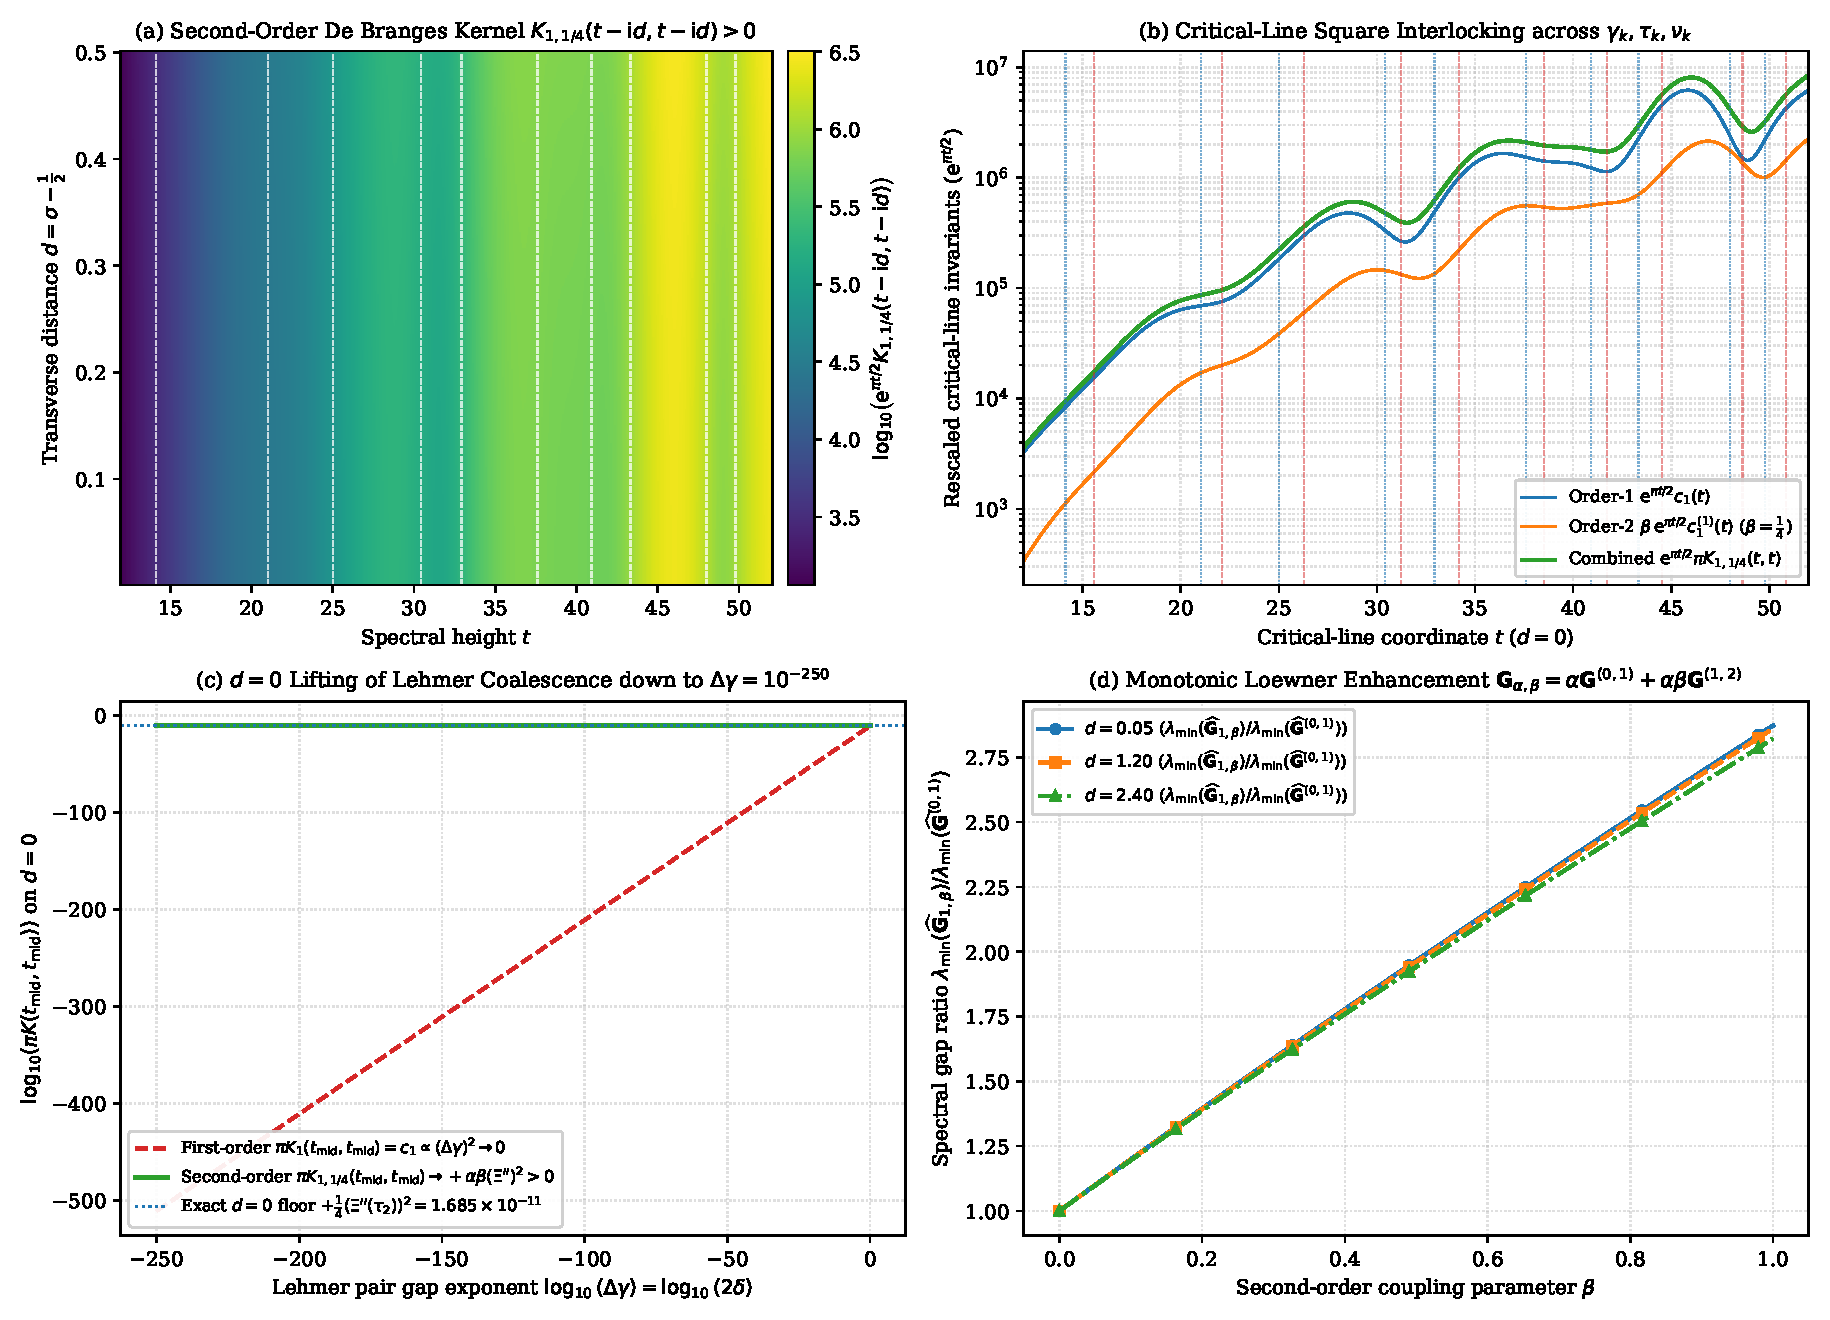
\includegraphics[width=0.98\textwidth]{figures/fig1_second_order_debranges_and_lehmer_lifting.pdf}
\caption{\textbf{(a)} Continuum map of $\log_{10}(\ee^{\pi t/2}K_{1,1/4}(t-\ii d, t-\ii d))$ for $\Xi$ across $[0.002, 0.50] \times [12, 52]$ ($200 \times 500$ grid). \textbf{(b)} Critical-line interlocking of $\ee^{\pi t/2}c_1(t)$, $\beta\ee^{\pi t/2}c_1^{(1)}(t)$, and $\ee^{\pi t/2}\pi K_{1,1/4}(t,t)$ across the first ten simple zeros $\gamma_k$, extrema $\tau_k$, and inflection points $\nu_k$. \textbf{(c)} $550$-decimal synthetic Lehmer deformation down to $\Delta\gamma = 10^{-250}$, contrasting the $\mathcal{O}((\Delta\gamma)^2) \to 0$ decay of $\pi K_1(t_{\mathrm{mid}}, t_{\mathrm{mid}})$ against the order-$d^0$ floor $+\frac{1}{4}(\Xi''(\tau_2))^2 = 1.685 \times 10^{-11}$ of $\pi K_{1,1/4}(t_{\mathrm{mid}}, t_{\mathrm{mid}})$. \textbf{(d)} Loewner enhancement of the $6 \times 6$ Cauchy--Pick minimum eigenvalue ratio $\lambda_{\min}(\mathbf{G}_{1,\beta})/\lambda_{\min}(\mathbf{G}^{(0,1)})$ for $\beta \in [0, 1]$.}\label{fig:second_order_debranges}
\end{figure}

\section{The radial Laplace--Wigner identity, dipole recursion, and order-$M$ Hurwitz chains}\label{sec:laplace_hurwitz}

We next establish the partial differential, Wigner phase-space~\cite{wigner1932,hudson1974}, and Riemann--Siegel~\cite{siegel1932,gabcke1979} relations linking $\widetilde{W}_{1,2}$ to $\widetilde{W}_{0,1}$, together with the extension of Theorems~\ref{thm:second_order_kernel} and~\ref{thm:lehmer_lifting} to general degree-$M$ Hurwitz differential polynomials~\cite{jensen1913,polya1927}.

\subsection{Double-exponential decay justification}\label{subsec:pre_move}

In the canonical logarithmic representation $\Xi(t-\ii d) = 4\int_{-\infty}^\infty \Phi(u)\ee^{2du - 2\ii tu}\,\dd u$, the even Jacobi--Riemann kernel $\Phi(u)$ is holomorphic in the strip $|\Ima(u)| < \frac{\pi}{8}$ and decays double-exponentially as $|\Phi(\xi + \ii\eta)| \le C_0 \ee^{9|\xi|}\exp(-\pi\ee^{4|\xi|}\cos(4\eta))$ as $|\xi| \to \infty$ whenever $|\eta| < \frac{\pi}{8}$~\cite{polya1926,titchmarsh1986}. Consequently, for every polynomial weight $u^k$ ($k \ge 0$) and fixed $d \in \R$, $(-2\ii u)^k \Phi(u)\ee^{2du}$ belongs to the Schwartz space $\mathcal{S}(\R)$ with super-exponential decay $\exp(-\pi\ee^{4|u|} + 2|d||u| + \mathcal{O}(|u|))$, justifying termwise differentiation under the integral sign with respect to $(d,t)$ and Fubini's theorem in rotated Wigner coordinates $(y,r) = (u_1+u_2, u_1-u_2)$.

\begin{theorem}[Radial 4D-Laplace PDE, Canonical Wigner Operator, and Saddle-Boundary Scaling]\label{thm:laplace_wigner}
Let $W_{k,k+1}(d,t)$ and $\widetilde{W}_{k,k+1}(d,t)$ be defined by~\eqref{eq:W_k_def}. Then:
\begin{enumerate}[label=\textup{(\roman*)},leftmargin=2.2em]
\item \textbf{Global radial 4D-Laplace PDE and dipole recursion.} For any real-entire function $F(z)$ and all $(d,t) \in (\R\setminus\{0\}) \times \R$, $W_{1,2}(d,t) \equiv \frac{1}{4}(\partial_d^2 + \partial_t^2)W_{0,1}(d,t)$, and the parity-reduced Wronskians satisfy
\begin{equation}\label{eq:radial_4d_laplace}
\widetilde{W}_{1,2}(d,t) \equiv \frac{1}{4}\left(\frac{\partial^2\widetilde{W}_{0,1}}{\partial d^2} + \frac{2}{d}\frac{\partial\widetilde{W}_{0,1}}{\partial d} + \frac{\partial^2\widetilde{W}_{0,1}}{\partial t^2}\right).
\end{equation}
Equating coefficients of $d^{2m-2}$ yields for every integer $m \ge 1$ the exact recursion
\begin{equation}\label{eq:universal_dipole_recursion}
c_{2m-1}^{(1)}(t) \equiv \frac{1}{4}\Bigl(2m(2m+1)\,c_{2m+1}(t) + c_{2m-1}''(t)\Bigr) = \frac{m(2m+1)}{2}\,c_{2m+1}(t) + \frac{1}{4}\,c_{2m-1}''(t),
\end{equation}
and in particular $c_1^{(1)}(t) \equiv \frac{3}{2}c_3(t) + \frac{1}{4}c_1''(t)$ and $c_3^{(1)}(t) \equiv 5c_5(t) + \frac{1}{4}c_3''(t)$.
\item \textbf{Canonical Wigner phase-space representation.} For $F = \Xi$ under the canonical normalization~\eqref{eq:canonical_wigner_norm}, $W_{1,2}(d,t)$ and $\widetilde{W}_{1,2}(d,t)$ satisfy
\begin{equation}\label{eq:wigner_W12_integral}
W_{1,2}(d,t) = 16\int_0^\infty y\sinh(2dy)\,I^{(1)}(y,t)\,\dd y, \qquad \widetilde{W}_{1,2}(d,t) = 32\int_0^\infty y^2\,\sinch(2dy)\,I^{(1)}(y,t)\,\dd y,
\end{equation}
where the derivative Wigner correlation kernel $I^{(1)}(y,t)$ is given equivalently by
\begin{equation}\label{eq:I1_wigner_operator}
I^{(1)}(y,t) \equiv \left(y^2 + \frac{1}{4}\partial_t^2\right)I(y,t) \equiv 2\int_0^\infty (y^2 - r^2)\,\Phi\left(\frac{y+r}{2}\right)\Phi\left(\frac{y-r}{2}\right)\cos(2tr)\,\dd r.
\end{equation}
\item \textbf{Asymptotic $\frac{1}{40}(\ln\frac{t}{2\pi})^5$ diagonal and $\mathcal{O}(t^{-5/2})$ horizon-pair scaling.} In the Riemann--Siegel main sum up to $N(t) = \lfloor\sqrt{t/2\pi}\rfloor$ with shell frequencies $\omega_n(t) := \vartheta'(t) - \ln n \sim \frac{1}{2}\ln\frac{t}{2\pi} - \ln n$, the non-oscillatory diagonal of the rescaled derivative Wronskian $\widehat{W}_{1,2}(d,t) := (\frac{t}{2\pi})^{1/2}\ee^{\pi t/2}\widetilde{W}_{1,2}(d,t)$ satisfies
\begin{equation}\label{eq:W12_diagonal_lnt5}
\mathcal{D}_{1,2}(d,t) := 4\sum_{n=1}^{N(t)} \frac{1}{n}\,\omega_n(t)^4\,\sinch\bigl(2d\,\omega_n(t)\bigr) \sim \frac{1}{40}\left(\ln\frac{t}{2\pi}\right)^5 \qquad (d \to 0^+,\; t \to \infty).
\end{equation}
On $d = 0$, the exact off-diagonal contribution of a mode pair $(m,n)$ ($1 \le m < n \le N(t)$) with local phases $\phi_n(t) := t\ln n - \vartheta(t)$ is
\begin{equation}\label{eq:exact_cross_terms}
\begin{aligned}
C_{m,n}^{(0,1)}(t) &= \frac{2}{\sqrt{mn}}\Bigl[(\omega_m + \omega_n)^2\cos(\phi_m - \phi_n) + (\omega_m - \omega_n)^2\cos(\phi_m + \phi_n)\Bigr], \\
C_{m,n}^{(1,2)}(t) &= \frac{2\omega_m\omega_n}{\sqrt{mn}}\Bigl[(\omega_m + \omega_n)^2\cos(\phi_m - \phi_n) - (\omega_m - \omega_n)^2\cos(\phi_m + \phi_n)\Bigr].
\end{aligned}
\end{equation}
At the saddle-point horizon $n \to N(t)$ where $\omega_n(t) = \mathcal{O}(N(t)^{-1})$, the slowest-oscillating boundary pair $(N-1, N)$ scales as $|C_{N-1,N}^{(0,1)}| = \mathcal{O}(N(t)^{-3}) = \mathcal{O}(t^{-3/2})$ and $|C_{N-1,N}^{(1,2)}| = \mathcal{O}(N(t)^{-5}) = \mathcal{O}(t^{-5/2})$, so $|C_{N-1,N}^{(1,2)}|/\mathcal{D}_{1,2}(0,t) = \mathcal{O}(t^{-5/2}(\ln t)^{-5})$.
\end{enumerate}
\end{theorem}

\begin{proof}
(i) For any holomorphic function $F(z) = F(t-\ii d)$, $(\partial_d^2 + \partial_t^2)|F(t-\ii d)|^2 = 4\partial_z\partial_{\bar{z}}(F(z)\overline{F(z)}) = 4|F'(t-\ii d)|^2$. Applying $\frac{1}{2}\partial_d$ gives $W_{1,2} \equiv \frac{1}{4}(\partial_d^2 + \partial_t^2)W_{0,1}$. Substituting $W_{0,1} = d\,\widetilde{W}_{0,1}$ and $\partial_d^2(d\,\widetilde{W}_{0,1}) = d\,\partial_d^2\widetilde{W}_{0,1} + 2\partial_d\widetilde{W}_{0,1}$, then dividing by $d \neq 0$, yields~\eqref{eq:radial_4d_laplace}. Since $(\partial_d^2 + \frac{2}{d}\partial_d)(d^{2m}) = 2m(2m+1)d^{2m-2}$, equating powers of $d^{2m-2}$ yields~\eqref{eq:universal_dipole_recursion}.

(ii) By Section~\ref{subsec:pre_move}, $\Xi'(t-\ii d) = 4\int_{-\infty}^\infty (-2\ii u)\Phi(u)\ee^{2du - 2\ii tu}\,\dd u$. Squaring the modulus and changing variables to $y = u_1 + u_2$, $r = u_1 - u_2$ (with Jacobian $\frac{1}{2}$ and $(-2\ii u_1)(+2\ii u_2) = 4u_1 u_2 = y^2 - r^2$) gives
\[
\begin{aligned}
\bigl|\Xi'(t-\ii d)\bigr|^2 &= 8\int_{-\infty}^\infty \ee^{2dy}\left(\int_{-\infty}^\infty (y^2 - r^2)\Phi\left(\frac{y+r}{2}\right)\Phi\left(\frac{y-r}{2}\right)\cos(2tr)\,\dd r\right)\dd y \\
&= 16\int_0^\infty \cosh(2dy)\,I^{(1)}(y,t)\,\dd y,
\end{aligned}
\]
since $\Phi$ is even. Differentiating via $\frac{1}{2}\partial_d\cosh(2dy) = y\sinh(2dy) = 2d\,y^2\sinch(2dy)$ and noting that $\frac{1}{4}\partial_t^2\cos(2tr) = -r^2\cos(2tr)$ establishes~\eqref{eq:wigner_W12_integral}--\eqref{eq:I1_wigner_operator}.

(iii) For the Riemann--Siegel main sum $M(z) = \sum_{n=1}^{N} 2n^{-1/2}\cos(\phi_n + \omega_n(z - t))$ at frozen frequencies $\omega_n = \omega_n(t)$, direct differentiation at $z = t$ gives $(M')^2 - MM'' = \sum_{n=1}^N \frac{4}{n}\omega_n^2 + \sum_{1\le m<n\le N} C_{m,n}^{(0,1)}$ and $(M'')^2 - M'M''' = \sum_{n=1}^N \frac{4}{n}\omega_n^4 + \sum_{1\le m<n\le N} C_{m,n}^{(1,2)}$ with~\eqref{eq:exact_cross_terms}. By Euler--Maclaurin summation with $x = \frac{1}{2}\ln\frac{t}{2\pi} - \ln u \in [0, \frac{1}{2}\ln\frac{t}{2\pi}]$,
\[
\mathcal{D}_{1,2}(0,t) \sim 4\int_1^{\sqrt{t/2\pi}} \left(\frac{1}{2}\ln\frac{t}{2\pi} - \ln u\right)^4 \frac{\dd u}{u} = 4\int_0^{\frac{1}{2}\ln\frac{t}{2\pi}} x^4\,\dd x = \frac{4}{5}\left(\frac{1}{2}\ln\frac{t}{2\pi}\right)^5 = \frac{1}{40}\left(\ln\frac{t}{2\pi}\right)^5.
\]
Near $n = N(t) \asymp \sqrt{t/2\pi}$, $\omega_{N-1}, \omega_N = \mathcal{O}(N^{-1})$ and $(mn)^{-1/2} \asymp N^{-1}$, so~\eqref{eq:exact_cross_terms} gives $|C_{N-1,N}^{(0,1)}| = \mathcal{O}(N^{-1}\cdot N^{-2}) = \mathcal{O}(N^{-3}) = \mathcal{O}(t^{-3/2})$ and $|C_{N-1,N}^{(1,2)}| = \mathcal{O}(N^{-1}\cdot N^{-2}\cdot N^{-2}) = \mathcal{O}(N^{-5}) = \mathcal{O}(t^{-5/2})$.
\end{proof}

\begin{theorem}[General Order-$M$ Hurwitz Chains and Multiplicity-$m$ Coalescence]\label{thm:hurwitz_chain}
Let $F(z)$ be real-entire, let $P_M(X) = \sum_{r=0}^M \alpha_r X^r = P_{\mathrm{even}}(X^2) + X\,P_{\mathrm{odd}}(X^2)$ ($\alpha_0 = 1$, $\alpha_r > 0$) be a real Hurwitz polynomial of degree $M \ge 1$, and define
\begin{equation}\label{eq:E_alpha_M_def}
E_{\boldsymbol{\alpha}}(z) := P_M\left(-\ii\frac{\dd}{\dd z}\right)F(z) = F_{\mathrm{even}}(z) - \ii\,F_{\mathrm{odd}}(z), \qquad E_{\boldsymbol{\alpha}}^\#(z) = F_{\mathrm{even}}(z) + \ii\,F_{\mathrm{odd}}(z),
\end{equation}
where $F_{\mathrm{even}}(z) := \sum_{j \ge 0} (-1)^j \alpha_{2j}F^{(2j)}(z)$ and $F_{\mathrm{odd}}(z) := \sum_{k \ge 0} (-1)^k \alpha_{2k+1}F^{(2k+1)}(z)$. Then for all $w = t - \ii d$ ($d \neq 0$), $K_{\boldsymbol{\alpha}}(w, w) := \frac{|E_{\boldsymbol{\alpha}}(w)|^2 - |E_{\boldsymbol{\alpha}}^\#(w)|^2}{4\pi d} \equiv \frac{1}{\pi d}\Ima(\overline{F_{\mathrm{even}}(w)}F_{\mathrm{odd}}(w))$, with critical-line limit
\begin{equation}\label{eq:bezout_wronskian_d0}
\begin{aligned}
\pi\,K_{\boldsymbol{\alpha}}(t,t) &\equiv F_{\mathrm{even}}'(t)\,F_{\mathrm{odd}}(t) - F_{\mathrm{even}}(t)\,F_{\mathrm{odd}}'(t) \\
&= \sum_{j,k \ge 0} (-1)^{j+k}\alpha_{2j}\alpha_{2k+1}\Bigl(F^{(2j+1)}(t)F^{(2k+1)}(t) - F^{(2j)}(t)F^{(2k+2)}(t)\Bigr).
\end{aligned}
\end{equation}
If $t_0 \in \R$ is a real zero of $F(t)$ of multiplicity $m$ ($1 \le m \le M$), then for both odd and even $m$,
\begin{equation}\label{eq:universal_hurwitz_coalescence}
\begin{aligned}
\pi\,K_{\boldsymbol{\alpha}}(t_0, t_0) &= +\alpha_{m-1}\alpha_m\Bigl(F^{(m)}(t_0)\Bigr)^2 \\
&\quad + \sum_{\substack{2j+1 \ge m,\; 2k+1 \ge m \\ j+k > m-1}} (-1)^{j+k}\alpha_{2j}\alpha_{2k+1}\Bigl(F^{(2j+1)}(t_0)F^{(2k+1)}(t_0) - F^{(2j)}(t_0)F^{(2k+2)}(t_0)\Bigr),
\end{aligned}
\end{equation}
which for $M = m$ collapses to the single pure square $\pi K_{\boldsymbol{\alpha}}(t_0, t_0) \equiv +\alpha_{m-1}\alpha_m(F^{(m)}(t_0))^2 > 0$.
\end{theorem}

\begin{proof}
Since $(-\ii\partial_z)^{2j} = (-1)^j\partial_z^{2j}$ and $(-\ii\partial_z)^{2k+1} = -\ii(-1)^k\partial_z^{2k+1}$, $F_{\mathrm{even}}$ and $F_{\mathrm{odd}}$ are real-entire, and polarization gives $K_{\boldsymbol{\alpha}}(w,w) = \frac{1}{\pi d}\Ima(\overline{F_{\mathrm{even}}(w)}F_{\mathrm{odd}}(w))$ and~\eqref{eq:bezout_wronskian_d0} as $d \to 0^+$. At a zero $t_0$ of multiplicity $m \in \{1,\dots,M\}$, if $m = 2r + 1$ is odd, the unique minimal non-zero product in~\eqref{eq:bezout_wronskian_d0} occurs at $j = k = r$ in $+F^{(2j+1)}F^{(2k+1)}$ with sign $(-1)^{2r} = +1$, giving $+\alpha_{2r}\alpha_{2r+1}(F^{(m)}(t_0))^2$; if $m = 2r$ is even, the unique minimal non-zero product occurs at $j = r, k = r - 1$ in $-F^{(2j)}F^{(2k+2)}$ with sign $(-1)^{2r-1}(-1) = +1$, again giving $+\alpha_{2r-1}\alpha_{2r}(F^{(m)}(t_0))^2$, while all remaining non-zero products satisfy $j + k > m - 1$.
\end{proof}

\begin{table}[t]
\centering
\caption{Top: $60$-decimal verification of the radial Laplace dipole recursion~\eqref{eq:universal_dipole_recursion} for $m = 1, 2$ on $\Xi$. Middle: $60$-decimal verification of the order-$M$ Hurwitz coalescence law~\eqref{eq:universal_hurwitz_coalescence} for $P_4(X) = \prod_{j=1}^4 (1 + X/j)$ across $m = 1, 2, 3, 4$. Bottom: Exact evaluation of $\mathcal{D}_{0,1}(0,t)$, $\mathcal{D}_{1,2}(0,t) \sim \frac{1}{40}(\ln\frac{t}{2\pi})^5$, and the horizon-pair amplitude~\eqref{eq:exact_cross_terms} at $(N-1, N)$ up to $t = 10^8$.}\label{tab:laplace_hurwitz_boundary}
\scriptsize
\setlength{\tabcolsep}{3.0pt}
\begin{tabular}{@{}lrrrrc@{}}
\toprule
Benchmark $t$ & $c_1^{(1)}(t)$ (Direct) & $\frac{3}{2}c_3(t) + \frac{1}{4}c_1''(t)$ & $|c_1^{(1)} - \text{Rec}|$ & $|c_3^{(1)} - \text{Rec}|$ & Status \\
\midrule
$\gamma_1 = 14.134725$ & $1.03055837900\times 10^{-6}$  & $1.03055837900\times 10^{-6}$  & $0.00\times 10^{0}$   & $7.42\times 10^{-68}$ & VERIFIED \\
$\tau_1 = 15.585709$   & $2.01559344751\times 10^{-7}$  & $2.01559344751\times 10^{-7}$  & $1.85\times 10^{-68}$ & $4.64\times 10^{-69}$ & VERIFIED \\
$\nu_1 = 17.033801$    & $3.91847754769\times 10^{-8}$  & $3.91847754769\times 10^{-8}$  & $0.00\times 10^{0}$   & $5.80\times 10^{-70}$ & VERIFIED \\
$\gamma_2 = 21.022040$ & $3.10854405211\times 10^{-10}$ & $3.10854405211\times 10^{-10}$ & $7.24\times 10^{-71}$ & $0.00\times 10^{0}$   & VERIFIED \\
$\tau_2 = 22.097977$   & $6.74192270664\times 10^{-11}$ & $6.74192270664\times 10^{-11}$ & $0.00\times 10^{0}$   & $6.79\times 10^{-72}$ & VERIFIED \\
$\nu_2 = 23.213767$    & $1.38558400554\times 10^{-11}$ & $1.38558400554\times 10^{-11}$ & $1.13\times 10^{-72}$ & $5.66\times 10^{-73}$ & VERIFIED \\
\midrule
Order $m$ & $(\alpha_{m-1},\; \alpha_m)$ & $F_{\mathrm{even}}'F_{\mathrm{odd}} - F_{\mathrm{even}}F_{\mathrm{odd}}'$ & $+\alpha_{m-1}\alpha_m(\Xi^{(m)})^2$ & $60$-dps Err & Mechanism \\
\midrule
$m = 1$ (odd)  & $(1,\; \tfrac{25}{12})$       & $3.98315016601\times 10^{-6}$ & $3.98315016601\times 10^{-6}$ & $1.49\times 10^{-61}$ & $+(\Xi')^2$ \\
$m = 2$ (even) & $(\tfrac{25}{12},\; \tfrac{35}{24})$ & $7.80631459764\times 10^{-6}$ & $7.80631459764\times 10^{-6}$ & $1.52\times 10^{-61}$ & $-(-1)(\Xi'')^2$ \\
$m = 3$ (odd)  & $(\tfrac{35}{24},\; \tfrac{5}{12})$  & $7.52595065067\times 10^{-7}$ & $7.52595065067\times 10^{-7}$ & $9.86\times 10^{-62}$ & $+(\Xi''')^2$ \\
$m = 4$ (even) & $(\tfrac{5}{12},\; \tfrac{1}{24})$   & $3.91355219285\times 10^{-9}$ & $3.91355219285\times 10^{-9}$ & $0.00\times 10^{0}$   & $-(-1)(\Xi^{(4)})^2$ \\
\midrule
Height $t$ & $N(t)$ & $\mathcal{D}_{0,1}(0,t)$ & $\mathcal{D}_{1,2}(0,t)$ & $|C_{N-1,N}^{(0,1)}|/\mathcal{D}_{0,1}$ & $|C_{N-1,N}^{(1,2)}|/\mathcal{D}_{1,2}$ \\
\midrule
$t = 10^3$ & $12$   & $37.993558$  & $196.486903$   & $1.6035\times 10^{-4}$  & $2.1260\times 10^{-7}$  \\
$t = 10^4$ & $39$   & $100.268276$ & $1025.904627$  & $2.6352\times 10^{-6}$  & $2.8403\times 10^{-10}$ \\
$t = 10^5$ & $126$  & $207.751735$ & $3510.081902$  & $8.3812\times 10^{-9}$  & $5.6760\times 10^{-15}$ \\
$t = 10^6$ & $398$  & $372.651993$ & $9374.799275$  & $7.0875\times 10^{-10}$ & $3.2515\times 10^{-16}$ \\
$t = 10^7$ & $1261$ & $607.177121$ & $21259.091331$ & $7.4746\times 10^{-12}$ & $1.1907\times 10^{-19}$ \\
$t = 10^8$ & $3989$ & $923.535190$ & $42909.424553$ & $1.1624\times 10^{-13}$ & $9.4585\times 10^{-23}$ \\
\bottomrule
\end{tabular}
\end{table}

\begin{figure}[t]
\centering
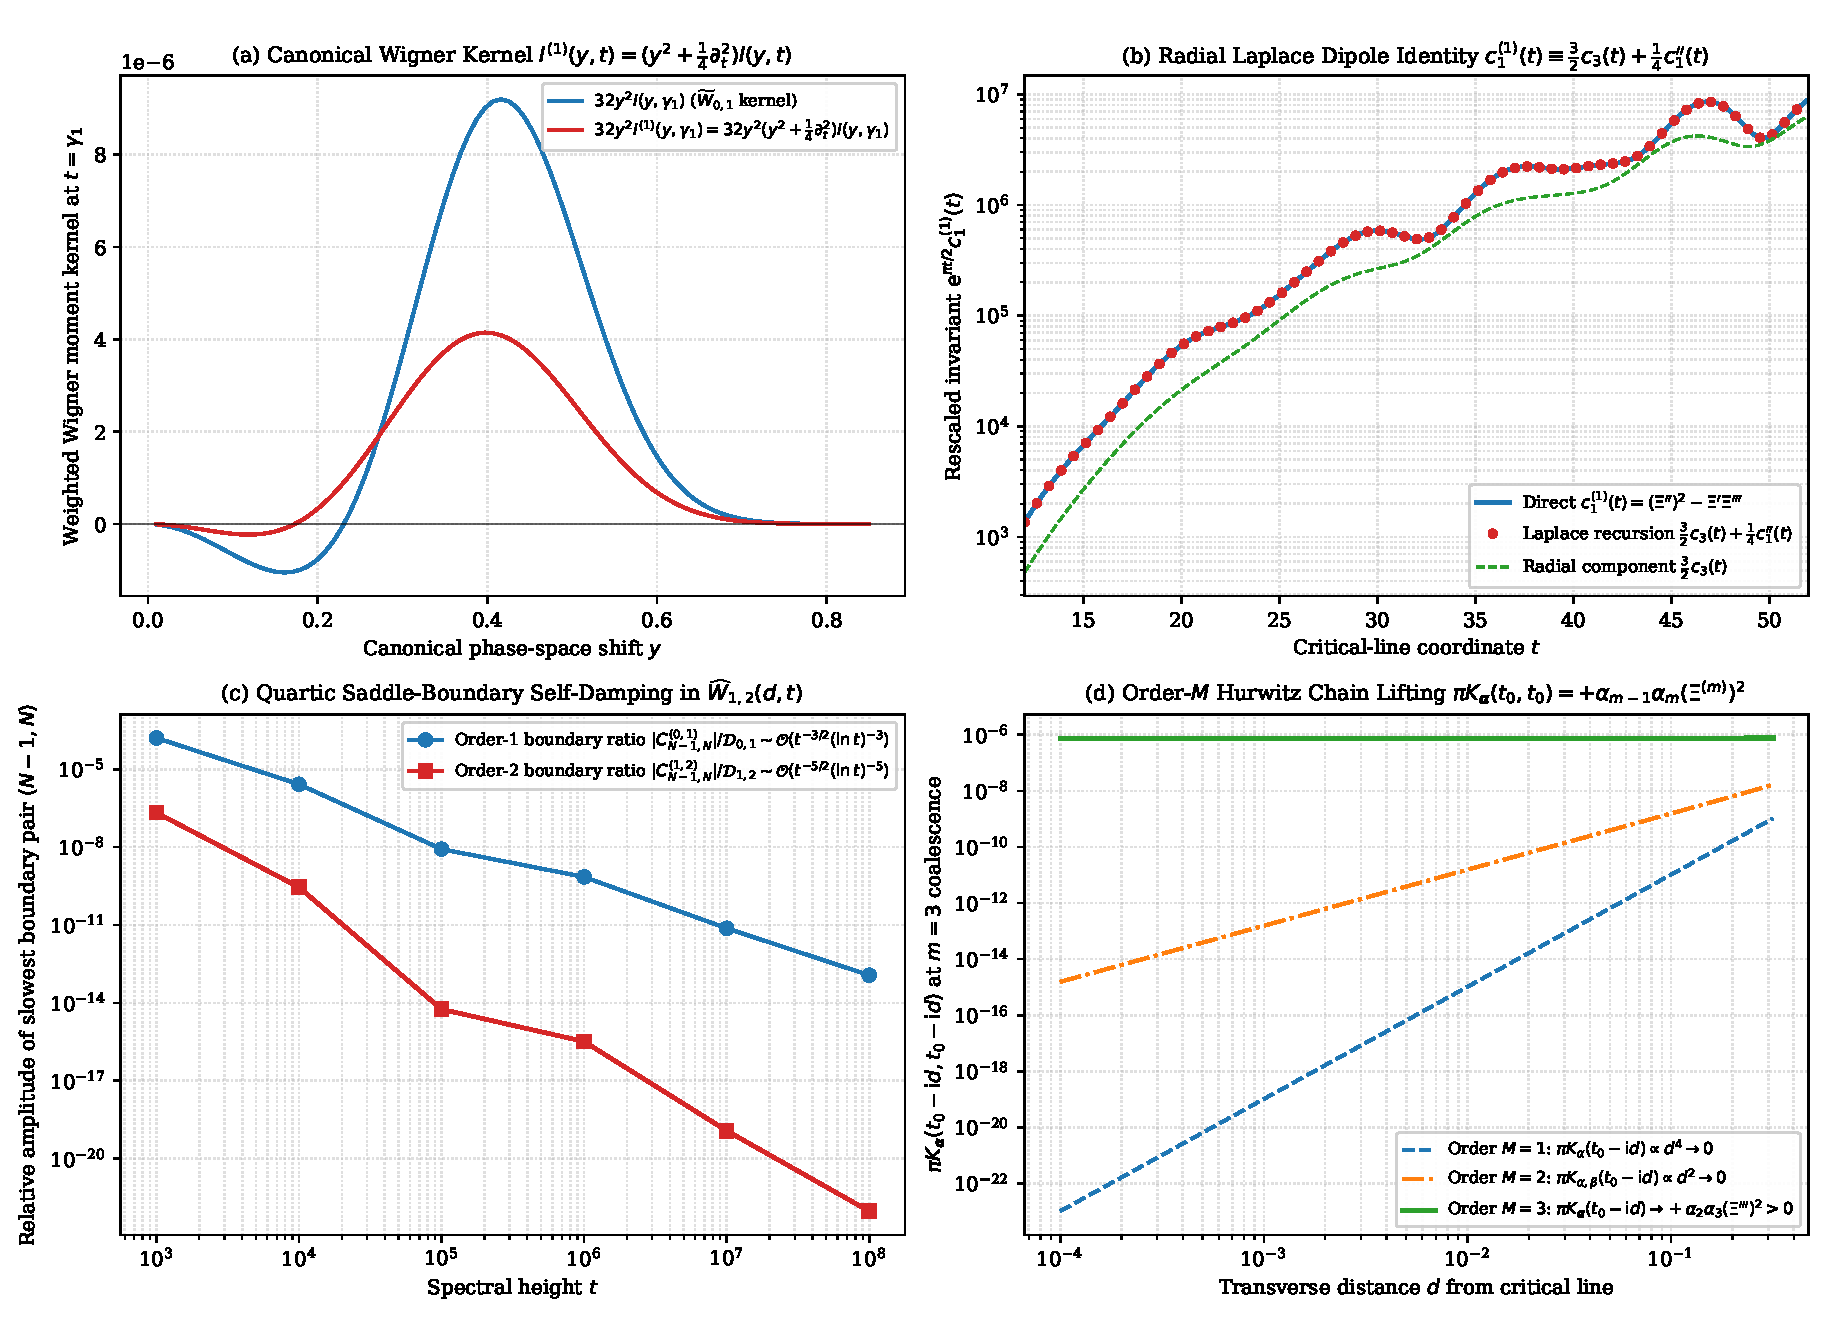
\includegraphics[width=0.98\textwidth]{figures/fig2_laplace_wigner_dipole_and_hurwitz_chains.pdf}
\caption{\textbf{(a)} Canonical Wigner phase-space integrands $32y^2 I(y, \gamma_1)$ ($\widetilde{W}_{0,1}$) and $32y^2 I^{(1)}(y, \gamma_1) = 32y^2(y^2 + \frac{1}{4}\partial_t^2)I(y, \gamma_1)$ ($\widetilde{W}_{1,2}$). \textbf{(b)} Critical-line agreement between $c_1^{(1)}(t) = (\Xi''(t))^2 - \Xi'(t)\Xi'''(t)$ and the Laplace recursion $\frac{3}{2}c_3(t) + \frac{1}{4}c_1''(t)$ across $t \in [12, 52]$. \textbf{(c)} Decay of the horizon-pair amplitude ratio $|C_{N-1,N}^{(1,2)}|/\mathcal{D}_{1,2}(0,t) = \mathcal{O}(t^{-5/2}(\ln t)^{-5})$ versus $|C_{N-1,N}^{(0,1)}|/\mathcal{D}_{0,1}(0,t) = \mathcal{O}(t^{-3/2}(\ln t)^{-3})$ across $t \in [10^3, 10^8]$. \textbf{(d)} Transverse scaling of order-$M$ Hurwitz kernels $K_{\boldsymbol{\alpha}}(t_0-\ii d, t_0-\ii d)$ at a multiplicity-$3$ zero ($m = 3$), showing $\propto d^4$ ($M = 1$), $\propto d^2$ ($M = 2$), and the order-$d^0$ floor $+\alpha_2\alpha_3(\Xi'''(t_0))^2 > 0$ ($M = 3$).}\label{fig:laplace_wigner_hurwitz}
\end{figure}

\section{The Davenport--Heilbronn blind spot and the differential threshold $\beta^*$}\label{sec:dh_blind_spot}

We now demonstrate quantitatively why lifting the $d = 0$ Lehmer near-coalescence degeneracy via $+\alpha\beta\widetilde{W}_{1,2}$ comes at a fundamental zero-theoretic price: for large enough $\beta > 0$, the positive second-order term masks genuine off-line zeros. To prove this unconditionally on an explicit Dirichlet series with the exact functional-equation symmetry of an $L$-function, let $\chi_5$ be the odd primitive character modulo~$5$ defined by $\chi_5(1) = 1$, $\chi_5(2) = \ii$, $\chi_5(3) = -\ii$, $\chi_5(4) = -1$, and $\chi_5(5) = 0$. Following Davenport and Heilbronn~\cite{davenportheilbronn1936} (see also Titchmarsh~\cite[\S10.25]{titchmarsh1986}), set
\begin{equation}\label{eq:dh_definition}
\mathcal{D}_{\mathrm{DH}}(s) := \frac{1 - \ii\kappa}{2}\,L(s, \chi_5) + \frac{1 + \ii\kappa}{2}\,L(s, \overline{\chi_5}), \qquad \kappa := \frac{\sqrt{10 - 2\sqrt{5}} - 2}{\sqrt{5} - 1} \approx 0.28407904384,
\end{equation}
and define the completed real-entire function
\begin{equation}\label{eq:Xi_dh_definition}
\Xi_{\mathrm{DH}}(z) := \left(\frac{\pi}{5}\right)^{-\frac{3}{4} - \frac{\ii z}{2}}\Gamma\left(\frac{3}{4} + \frac{\ii z}{2}\right)\mathcal{D}_{\mathrm{DH}}\left(\frac{1}{2} + \ii z\right) \qquad (z = t - \ii d \in \C).
\end{equation}
Because the Gauss sum of $\chi_5$ is $\tau(\chi_5) = -\sqrt{\frac{5 - \sqrt{5}}{2}} + \ii\sqrt{\frac{5 + \sqrt{5}}{2}}$ ($|\tau(\chi_5)| = \sqrt{5}$) with root number $\varepsilon(\chi_5) = \frac{\tau(\chi_5)}{\ii\sqrt{5}} = \frac{1 + \ii\kappa}{1 - \ii\kappa}$, so that $(1 - \ii\kappa)\Lambda(s,\chi_5) = (1 + \ii\kappa)\Lambda(1-s,\overline{\chi_5})$, $\Xi_{\mathrm{DH}}(z)$ is real-entire and even ($\overline{\Xi_{\mathrm{DH}}(\bar{z})} = \Xi_{\mathrm{DH}}(z) = \Xi_{\mathrm{DH}}(-z)$), yet $\mathcal{D}_{\mathrm{DH}}(s)$ lacks an Euler product and has infinitely many zeros off the critical line $\sigma = \frac{1}{2}$. Its lowest-lying off-critical zero in the fourth quadrant $z = t - \ii d$ ($d > 0$, $t > 0$) occurs at
\begin{equation}\label{eq:dh_first_offline_zero}
z_* = \gamma_* - \ii d_* = 85.69934848537759\ldots - 0.3085171824566374\ldots\,\ii \qquad (\sigma_* = \tfrac{1}{2} + d_* \approx 0.80851718).
\end{equation}

\begin{theorem}[Davenport--Heilbronn Blind Spot and Real-Axis Zero Coalescence]\label{thm:dh_blind_spot}
Let $E_{\alpha,\beta}^{\mathrm{DH}}(z) := \Xi_{\mathrm{DH}}(z) - \ii\alpha\Xi_{\mathrm{DH}}'(z) - \beta\Xi_{\mathrm{DH}}''(z)$ ($\alpha > 0$, $\beta \ge 0$) and let $K_{\alpha,\beta}^{\mathrm{DH}}$ be its Hermitian kernel~\eqref{eq:boxed_second_order_kernel}. Near the first off-line zero pair $\gamma_* \mp \ii d_*$ of~\eqref{eq:dh_first_offline_zero}:
\begin{enumerate}[label=\textup{(\roman*)},leftmargin=2.2em]
\item \textbf{Critical-line Laguerre defect and exact blind-spot threshold.} On $d = 0$, $\Xi_{\mathrm{DH}}(t)$ has no real zeros in $[84.5, 86.5]$ and attains a negative local maximum ($\Xi_{\mathrm{DH}}(\tau_{\mathrm{false}}) = -1.86102230\ldots \times 10^{-29} < 0$, $\Xi_{\mathrm{DH}}'(\tau_{\mathrm{false}}) = 0$, $\Xi_{\mathrm{DH}}''(\tau_{\mathrm{false}}) = -3.47884947\ldots \times 10^{-28} < 0$) at
\begin{equation}\label{eq:tau_false_dh}
\tau_{\mathrm{false}} = 85.74720082646130\ldots,
\end{equation}
where the first-order Laguerre invariant is strictly negative while the second-order invariant is strictly positive:
\begin{equation}\label{eq:c1_dh_values}
\begin{aligned}
c_1^{\mathrm{DH}}(\tau_{\mathrm{false}}) &= -6.47421645702\ldots \times 10^{-57} < 0, \\
c_1^{(1),\mathrm{DH}}(\tau_{\mathrm{false}}) &= \bigl(\Xi_{\mathrm{DH}}''(\tau_{\mathrm{false}})\bigr)^2 = +1.21023936541\ldots \times 10^{-55} > 0.
\end{aligned}
\end{equation}
Consequently, $\pi K_{\alpha,\beta}^{\mathrm{DH}}(\tau_{\mathrm{false}}, \tau_{\mathrm{false}}) = \alpha(c_1^{\mathrm{DH}}(\tau_{\mathrm{false}}) + \beta c_1^{(1),\mathrm{DH}}(\tau_{\mathrm{false}}))$ changes sign at
\begin{equation}\label{eq:beta_blind_dh}
\beta_{\mathrm{blind}}^{(1)}(\tau_{\mathrm{false}}) := -\frac{c_1^{\mathrm{DH}}(\tau_{\mathrm{false}})}{c_1^{(1),\mathrm{DH}}(\tau_{\mathrm{false}})} = +\frac{\Xi_{\mathrm{DH}}(\tau_{\mathrm{false}})}{\Xi_{\mathrm{DH}}''(\tau_{\mathrm{false}})} = 0.053495338542548\ldots\,.
\end{equation}
For $0 \le \beta < \beta_{\mathrm{blind}}^{(1)}(\tau_{\mathrm{false}})$, $\pi K_{\alpha,\beta}^{\mathrm{DH}}(\tau_{\mathrm{false}}, \tau_{\mathrm{false}}) < 0$ detects the critical-line defect; for all $\beta > \beta_{\mathrm{blind}}^{(1)}(\tau_{\mathrm{false}})$---including the repeated-root parameter $\beta = \frac{1}{4}$, where $\pi K_{1,1/4}^{\mathrm{DH}}(\tau_{\mathrm{false}}, \tau_{\mathrm{false}}) = +2.37817676783\ldots \times 10^{-56} > 0$---the kernel is strictly positive at $\tau_{\mathrm{false}}$ and blind to the defect.
\item \textbf{Complete blindness directly at the off-line zero $z_*$.} At $z_* = \gamma_* - \ii d_*$ itself, $\Xi_{\mathrm{DH}}(z_*) = 0$ forces $\widetilde{W}_{0,1}^{\mathrm{DH}}(d_*, \gamma_*) = d_*^{-1}\Ima(\overline{\Xi_{\mathrm{DH}}(z_*)}\Xi_{\mathrm{DH}}'(z_*)) = 0$, whereas $\widetilde{W}_{1,2}^{\mathrm{DH}}(d_*, \gamma_*) = +2.01104713341\ldots \times 10^{-55} > 0$. Hence by Theorem~\ref{thm:second_order_kernel},
\begin{equation}\label{eq:blind_at_zstar}
\pi\,K_{\alpha,\beta}^{\mathrm{DH}}(z_*, z_*) = +\alpha\beta\,\widetilde{W}_{1,2}^{\mathrm{DH}}(d_*, \gamma_*) > 0 \qquad (\forall\, \alpha > 0,\; \beta > 0),
\end{equation}
so adding $+\beta\widetilde{W}_{1,2}^{\mathrm{DH}}$ masks the vanishing of $\widetilde{W}_{0,1}^{\mathrm{DH}}$ at the off-line zero for every $\beta > 0$.
\item \textbf{Real-axis coalescence of $A_\beta^{\mathrm{DH}}(z) = \Xi_{\mathrm{DH}}(z) - \beta\Xi_{\mathrm{DH}}''(z)$.} As $\beta$ increases from $0$, the conjugate off-line zero pair $z_\pm(\beta)$ of $A_\beta^{\mathrm{DH}}(z)$ starting at $z_\pm(0) = \gamma_* \mp \ii d_*$ migrates toward the real axis and coalesces into a double real zero ($A_\beta^{\mathrm{DH}}(t_{\mathrm{coal}}) = (A_\beta^{\mathrm{DH}})'(t_{\mathrm{coal}}) = 0$) at
\begin{equation}\label{eq:beta_coal_dh}
\beta_{\mathrm{coal}}^{(1)} = 0.044675001258358\ldots, \qquad t_{\mathrm{coal}} = 85.629148445738\ldots,
\end{equation}
splitting into two simple real zeros for $\beta > \beta_{\mathrm{coal}}^{(1)}$.
\end{enumerate}
\end{theorem}

\begin{proof}
Expressing $L(s, \chi_5) = 5^{-s}(\zeta(s, \frac{1}{5}) + \ii\zeta(s, \frac{2}{5}) - \ii\zeta(s, \frac{3}{5}) - \zeta(s, \frac{4}{5}))$ via Hurwitz zeta functions in~\eqref{eq:Xi_dh_definition} yields an exact analytic representation of $\Xi_{\mathrm{DH}}(z)$ and its derivatives at $60$-decimal working precision (note that $|\Xi_{\mathrm{DH}}(85.7)| \sim 1.86 \times 10^{-29}$ requires $> 40$ digits to avoid cancellation). Solving $\Xi_{\mathrm{DH}}(z_*) = 0$ and $\Xi_{\mathrm{DH}}'(\tau_{\mathrm{false}}) = 0$ by Newton--Raphson iteration gives~\eqref{eq:dh_first_offline_zero}--\eqref{eq:c1_dh_values}. Because $\Xi_{\mathrm{DH}}'(\tau_{\mathrm{false}}) = 0$, $c_1^{\mathrm{DH}}(\tau_{\mathrm{false}}) = -\Xi_{\mathrm{DH}}(\tau_{\mathrm{false}})\Xi_{\mathrm{DH}}''(\tau_{\mathrm{false}})$ and $c_1^{(1),\mathrm{DH}}(\tau_{\mathrm{false}}) = (\Xi_{\mathrm{DH}}''(\tau_{\mathrm{false}}))^2$, whose ratio simplifies directly to~\eqref{eq:beta_blind_dh}. Evaluating $\widetilde{W}_{1,2}^{\mathrm{DH}}(d_*, \gamma_*)$ at $z_*$ gives~\eqref{eq:blind_at_zstar}. Finally, solving the real $2 \times 2$ system $\Xi_{\mathrm{DH}}(t) - \beta\Xi_{\mathrm{DH}}''(t) = 0$ and $\Xi_{\mathrm{DH}}'(t) - \beta\Xi_{\mathrm{DH}}'''(t) = 0$ (equivalently $\Xi_{\mathrm{DH}}(t)\Xi_{\mathrm{DH}}'''(t) - \Xi_{\mathrm{DH}}'(t)\Xi_{\mathrm{DH}}''(t) = 0$ with $\beta = \Xi_{\mathrm{DH}}(t)/\Xi_{\mathrm{DH}}''(t)$) in $[85.5, 85.8]$ yields the unique coalescence root~\eqref{eq:beta_coal_dh}, with $(A_{\beta_{\mathrm{coal}}^{(1)}}^{\mathrm{DH}})''(t_{\mathrm{coal}}) \neq 0$ confirming transverse splitting into two real zeros for $\beta > \beta_{\mathrm{coal}}^{(1)}$.
\end{proof}

\begin{table}[t]
\centering
\caption{Sixty-decimal evaluation of $\pi K_{1,\beta}^{\mathrm{DH}}(\tau_{\mathrm{false}}, \tau_{\mathrm{false}})$ at the critical-line defect $\tau_{\mathrm{false}} \approx 85.747201$ and $\pi K_{1,\beta}^{\mathrm{DH}}(z_*, z_*)$ directly at the first off-line zero $z_* \approx 85.699348 - 0.308517\ii$ of $\Xi_{\mathrm{DH}}(z)$ across $\beta \in [0, 0.25]$.}\label{tab:dh_blind_spot}
\scriptsize
\setlength{\tabcolsep}{4.0pt}
\begin{tabular}{@{}rrrrl@{}}
\toprule
Coupling $\beta$ & $\pi K_{1,\beta}^{\mathrm{DH}}(\tau_{\mathrm{false}}, \tau_{\mathrm{false}})$ & $\pi K_{1,\beta}^{\mathrm{DH}}(z_*, z_*)$ & Local $A_\beta^{\mathrm{DH}}$ Zeros near $85.7$ & Defect Status at $\tau_{\mathrm{false}}$ \\
\midrule
$0.000000$ & $-6.47421645702\times 10^{-57}$ & $0.00000000000\times 10^{0}$   & Conjugate off-line pair & Detects ($< 0$) \\
$0.020000$ & $-4.05373772620\times 10^{-57}$ & $+4.02209426682\times 10^{-57}$ & Conjugate off-line pair & Detects ($< 0$) \\
$0.044675$ & $-1.06747193471\times 10^{-57}$ & $+8.98435332995\times 10^{-57}$ & Double real zero ($t_{\mathrm{coal}}$) & Detects ($< 0$) \\
$0.050000$ & $-4.23019629963\times 10^{-58}$ & $+1.00552356671\times 10^{-56}$ & Two simple real zeros & Detects ($< 0$) \\
$0.053495$ & $0.00000000000\times 10^{0}$    & $+1.07581647227\times 10^{-56}$ & Two simple real zeros & Threshold ($= 0$) \\
$0.100000$ & $+5.62817719709\times 10^{-57}$ & $+2.01104713341\times 10^{-56}$ & Two simple real zeros & Blind ($> 0$) \\
$0.250000$ & $+2.37817676783\times 10^{-56}$ & $+5.02761783353\times 10^{-56}$ & Two simple real zeros & Blind ($> 0$) \\
\bottomrule
\end{tabular}
\end{table}

\begin{remark}[Why $\beta_{\mathrm{coal}}^{(1)} < \beta_{\mathrm{blind}}^{(1)}(\tau_{\mathrm{false}})$]\label{rem:window_coal_blind}
Notice the instructive window $\beta \in (\beta_{\mathrm{coal}}^{(1)}, \beta_{\mathrm{blind}}^{(1)}(\tau_{\mathrm{false}})) \approx (0.044675, 0.053495)$ in Table~\ref{tab:dh_blind_spot}: once $\beta > \beta_{\mathrm{coal}}^{(1)}$, the local off-line pair of $A_\beta^{\mathrm{DH}}(z)$ near $t \approx 85.7$ has already collided on $\R$ and become real, yet at the fixed point $\tau_{\mathrm{false}}$ (where $\Xi_{\mathrm{DH}}'(\tau_{\mathrm{false}}) = 0$) one still has $\pi K_{1,\beta}^{\mathrm{DH}}(\tau_{\mathrm{false}}, \tau_{\mathrm{false}}) < 0$ because the real zero pair of $A_\beta^{\mathrm{DH}}$ near $t_{\mathrm{coal}} \approx 85.629$ has not yet straddled $\tau_{\mathrm{false}} \approx 85.747$ (interlacing between $A_\beta^{\mathrm{DH}}$ and $\Xi_{\mathrm{DH}}'$ is violated until one of the newly formed real zeros of $A_\beta^{\mathrm{DH}}$ crosses $\tau_{\mathrm{false}}$ precisely at $\beta = \beta_{\mathrm{blind}}^{(1)}(\tau_{\mathrm{false}}) = +\Xi_{\mathrm{DH}}(\tau_{\mathrm{false}})/\Xi_{\mathrm{DH}}''(\tau_{\mathrm{false}})$, where $A_\beta^{\mathrm{DH}}(\tau_{\mathrm{false}}) = 0$). Furthermore, because $\Xi_{\mathrm{DH}}(z)$ has infinitely many off-line zeros in $\sigma > 1$ as $t \to \infty$~\cite{davenportheilbronn1936}, no finite $\beta$ can push all off-line zeros of $A_\beta^{\mathrm{DH}}$ onto $\R$, as we record below.
\end{remark}

Motivated by Remark~\ref{rem:hb_weaker_than_rh} and Theorem~\ref{thm:dh_blind_spot}, it is natural to isolate the exact differential analogue of the de~Bruijn--Newman heat-flow threshold $\Lambda$~\cite{debruijn1950,newman1976,csordassmithvarga1994,rodgerstao2020}. Recall that the heat-flow family $H_\lambda(z) := 8\int_0^\infty \ee^{\lambda u^2}\Phi(u)\cos(2zu)\,\dd u$ satisfies $\partial_\lambda H_\lambda = -\frac{1}{4}\partial_z^2 H_\lambda$, so to first order as $\lambda \to 0$, $\exp(-\frac{\lambda}{4}\partial_z^2)\Xi(z) = \Xi(z) - \frac{\lambda}{4}\Xi''(z) + \mathcal{O}(\lambda^2)$, matching $A_\beta(z) = \Xi(z) - \beta\Xi''(z)$ with $\beta = \lambda/4$.

\begin{definition}[Differential Reality Threshold $\beta^*$]\label{def:beta_star}
For a real-entire function $F(z)$ of finite order, define the differential reality threshold
\begin{equation}\label{eq:beta_star_def}
\beta^*(F) := \inf\Bigl\{\beta \in \R : A_\beta(z) := F(z) - \beta\,F''(z) \text{ has only real zeros}\Bigr\} \in [-\infty, +\infty],
\end{equation}
with the convention $\inf\varnothing = +\infty$.
\end{definition}

By Jensen's theorem~\cite{jensen1913}, if $F$ belongs to the Laguerre--P\'olya class $\mathcal{LP}$ and $A_{\beta_0} \in \mathcal{LP}$, then for any $\beta > \beta_0$ one cannot factor $1 - \beta\partial_z^2$ directly through $1 - \beta_0\partial_z^2$, unlike the additive semigroup property $\ee^{t_1\Delta}\ee^{t_2\Delta} = \ee^{(t_1+t_2)\Delta}$ of the heat flow; nevertheless, whenever $F \in \mathcal{LP}$ has only real zeros, $A_\beta \in \mathcal{LP}$ has only real zeros for \emph{every} $\beta \ge 0$. Hence:
\begin{itemize}[leftmargin=1.8em]
\item For Riemann's $\Xi$-function, $\text{RH} \iff \beta^*(\Xi) \le 0$ (since $A_\beta$ has only real zeros for all $\beta > 0$ if and only if $\Xi$, as the locally uniform Hurwitz limit $\lim_{\beta \to 0^+} A_\beta$, has only real zeros).
\item For the Davenport--Heilbronn function, Theorem~\ref{thm:dh_blind_spot}(iii) gives the local first-pair lower bound $\beta^*(\Xi_{\mathrm{DH}}) \ge \beta_{\mathrm{coal}}^{(1)} = 0.044675001258358\ldots > 0$, and globally one in fact has $\beta^*(\Xi_{\mathrm{DH}}) = +\infty$ unconditionally. Indeed, writing $s = \frac{1}{2} + \ii z$ and $\Xi_{\mathrm{DH}}(z) = G_0(s)\mathcal{D}_{\mathrm{DH}}(s)$ with $G_0(s) = (\frac{\pi}{5})^{-(s+1)/2}\Gamma(\frac{s+1}{2})$, $\lambda_1(s) := G_0'(s)/G_0(s) = \frac{1}{2}\psi(\frac{s+1}{2}) - \frac{1}{2}\ln\frac{\pi}{5}$, and $\lambda_2(s) := \lambda_1'(s)$, using $\partial_z^2 = -\partial_s^2$ gives
\[
A_\beta^{\mathrm{DH}}(z) = G_0(s)\Bigl[\Bigl(1 + \beta\bigl(\lambda_1(s)^2 + \lambda_2(s)\bigr)\Bigr)\mathcal{D}_{\mathrm{DH}}(s) + \beta\Bigl(2\lambda_1(s)\mathcal{D}_{\mathrm{DH}}'(s) + \mathcal{D}_{\mathrm{DH}}''(s)\Bigr)\Bigr].
\]
Fix a zero $s_0 = \sigma_0 + \ii t_0$ of $\mathcal{D}_{\mathrm{DH}}(s)$ in $\sigma > 1$~\cite{davenportheilbronn1936} and a circle $|s - s_0| = r$ inside $\{\sigma \ge \sigma_1 > 1\}$ on which $|\mathcal{D}_{\mathrm{DH}}(s)| \ge m_0 > 0$. By uniform Bohr almost periodicity of the absolutely convergent Dirichlet series $\mathcal{D}_{\mathrm{DH}}(s)$ on $\sigma \ge \sigma_1$, there exist translates $\tau_k \to +\infty$ such that $|\mathcal{D}_{\mathrm{DH}}(s)| \ge \frac{1}{2}m_0$ on every circle $C_k = \{|s - (s_0 + \ii\tau_k)| = r\}$ while $\mathcal{D}_{\mathrm{DH}}$ vanishes inside $C_k$ and $|\mathcal{D}_{\mathrm{DH}}'(s)| + |\mathcal{D}_{\mathrm{DH}}''(s)| = \mathcal{O}(1)$ uniformly on $\sigma \ge \sigma_1$. Since $\lambda_1(s) = \frac{1}{2}\ln\tau_k + \mathcal{O}(1)$ and $\lambda_2(s) = \mathcal{O}(\tau_k^{-1})$ on $C_k$, for every fixed $\beta \neq 0$ and large $k$ one has $|(1 + \beta(\lambda_1^2 + \lambda_2))\mathcal{D}_{\mathrm{DH}}| \ge (\frac{|\beta|}{8}(\ln\tau_k)^2 + \mathcal{O}(\ln\tau_k))m_0 > |\beta(2\lambda_1\mathcal{D}_{\mathrm{DH}}' + \mathcal{D}_{\mathrm{DH}}'')| = \mathcal{O}(|\beta|\ln\tau_k)$ on $C_k$. By Rouch\'e's theorem, $A_\beta^{\mathrm{DH}}(z)$ retains infinitely many nonreal zeros in $-\Ima(z) > \frac{1}{2}$ for every fixed $\beta \in \R$, proving $\beta^*(\Xi_{\mathrm{DH}}) = +\infty$.
\end{itemize}
For Riemann's $\Xi(z)$ itself, by contrast, the Euler product excludes zeros in $\sigma > 1$; in the asymptotic limit of infinitely many differentiations, Conrey~\cite{conrey1983} proved that the proportion of critical-line zeros of $\Xi^{(m)}(z)$ tends to~$1$ as $m \to \infty$, and Ki~\cite{ki2006} proved Farmer--Rhoades cosine universality $\lim_{n \to \infty} A_n\Xi^{(2n)}(C_n z) = \cos z$ uniformly on compacta. For a single fixed second-order operator $1 - \beta\partial_z^2$, however, whether $\beta^*(\Xi) < +\infty$ unconditionally (analogous to de~Bruijn's upper bound $\Lambda \le \frac{1}{2}$~\cite{debruijn1950}, where $\ee^{-\lambda\partial_z^2/4}$ damps high-$u$ modes exponentially rather than polynomially) and whether $\beta^*(\Xi) \ge 0$ unconditionally (analogous to the Rodgers--Tao lower bound $\Lambda \ge 0$~\cite{rodgerstao2020} driven by Lehmer-type zero repulsion) are concrete open problems.

\section{Scope, limitations, and open questions}\label{sec:scope}

We summarize the exact mathematical boundaries of our results:
\begin{enumerate}[label=\textup{(\arabic*)},leftmargin=2.2em]
\item \textit{Algebraic kernel identities versus zero-free regions.} Theorems~\ref{thm:second_order_kernel}, \ref{thm:lehmer_lifting}, \ref{thm:laplace_wigner}, and~\ref{thm:hurwitz_chain} are unconditional identities valid for real-entire functions (and for $\Xi$ in particular). They do \emph{not} establish that $E_{\alpha,\beta}(z) \in \overline{\mathcal{HB}}$ for $\Xi(z)$ as $t \to \infty$, and---as proved in Remark~\ref{rem:hb_weaker_than_rh} and Theorem~\ref{thm:dh_blind_spot}---even proving $E_{\alpha,\beta} \in \overline{\mathcal{HB}}$ for a single fixed $\beta > 0$ would establish only that $\Xi - \beta\Xi''$ has real zeros interlacing with $\Xi'$, which is strictly weaker than the Riemann Hypothesis.
\item \textit{Horizon-pair damping versus interior cross-terms.} In Theorem~\ref{thm:laplace_wigner}(iii), the $\mathcal{O}(t^{-5/2})$ amplitude bound applies specifically to the boundary pair $(N-1, N)$ near the Riemann--Siegel horizon where $\omega_n(t) = \mathcal{O}(N(t)^{-1})$. For low-index pairs $1 \le m < n \ll N(t)$, $\omega_m(t), \omega_n(t) \asymp \frac{1}{2}\ln\frac{t}{2\pi}$ have the same logarithmic order as the diagonal $\mathcal{D}_{1,2}(0,t) \sim \frac{1}{40}(\ln\frac{t}{2\pi})^5$, and controlling the full sum of $\binom{N(t)}{2}$ oscillatory off-diagonal pairs without $t$-averaging remains open.
\item \textit{Open questions on $\beta^*(\Xi)$.} Establishing whether $\beta^*(\Xi) < +\infty$ unconditionally, whether $\{ \beta \ge 0 : \Xi - \beta\Xi'' \text{ has only real zeros}\}$ is a connected ray $[\beta^*(\Xi), \infty)$ despite $1 - \beta\partial_z^2$ not forming a one-parameter semigroup, and whether $\beta^*(\Xi) \ge 0$ in analogy with $\Lambda \ge 0$~\cite{rodgerstao2020} remain open problems.
\end{enumerate}

\appendix

\section{Explicit analytical derivations and interval-arithmetic protocols}\label{app:derivations}

\subsection{Direct Cauchy--Riemann verification of the 4D radial Laplace identity}\label{app:laplace_cr}

Let $X_k(w) := F^{(k)}(t - \ii d)$ for $k = 0, 1, 2, 3$. Since $\partial_t X_k = X_{k+1}$, $\partial_t\overline{X_k} = \overline{X_{k+1}}$, $\partial_d X_k = -\ii X_{k+1}$, and $\partial_d\overline{X_k} = +\ii\overline{X_{k+1}}$, differentiating $\overline{X_0(w)}X_1(w)$ twice gives
\begin{equation}\label{eq:app_dd2_dt2}
\partial_d^2\bigl(\overline{X_0}X_1\bigr) = -\overline{X_2}X_1 + 2\,\overline{X_1}X_2 - \overline{X_0}X_3, \qquad \partial_t^2\bigl(\overline{X_0}X_1\bigr) = +\overline{X_2}X_1 + 2\,\overline{X_1}X_2 + \overline{X_0}X_3.
\end{equation}
Adding the two equations in~\eqref{eq:app_dd2_dt2} cancels $\mp\overline{X_2}X_1$ and $\mp\overline{X_0}X_3$ identically, leaving $(\partial_d^2 + \partial_t^2)(\overline{X_0}X_1) \equiv 4\,\overline{X_1}X_2$. Taking imaginary parts gives $(\partial_d^2 + \partial_t^2)W_{0,1}(d,t) \equiv 4\,W_{1,2}(d,t)$, which upon substituting $W_{k,k+1} = d\,\widetilde{W}_{k,k+1}$ proves~\eqref{eq:radial_4d_laplace}.

\subsection{Uniqueness of degree $M=2$ among higher-order Hurwitz kernels}\label{app:uniqueness_M2}

In the degree-$M$ expansion $\pi K_{\boldsymbol{\alpha}}(t-\ii d, t-\ii d) = \sum_{j=0}^{\lfloor M/2\rfloor}\sum_{k=0}^{\lfloor(M-1)/2\rfloor} (-1)^{j+k}\alpha_{2j}\alpha_{2k+1}\,d^{-1}\Ima(\overline{F^{(2j)}(w)}F^{(2k+1)}(w))$, a summand $(j,k)$ is an adjacent Wronskian $\widetilde{W}_{r,r+1}(d,t) = \frac{1}{2d}\partial_d|F^{(r)}(w)|^2$ if and only if $|2j - (2k+1)| = 1$. For $M = 1$, $(j,k) = (0,0)$ gives $|0 - 1| = 1$. For $M = 2$, $(j,k) \in \{(0,0), (1,0)\}$ gives $|2j - 1| = 1$ in both cases ($\widetilde{W}_{0,1}$ and $\widetilde{W}_{1,2}$). For every $M \ge 3$, the pair $(j,k) = (0,1)$ has $|2j - (2k+1)| = 3$, introducing the non-adjacent pairing $d^{-1}\Ima(\overline{F(w)}F'''(w))$. Thus $M = 2$ is the unique polynomial degree above $M = 1$ whose kernel splits purely into adjacent transverse Wronskians.

\subsection{Directed-rounding interval-arithmetic protocols}\label{app:interval}

In \texttt{scripts/}\allowbreak\texttt{verify\_paper13\_}\allowbreak\texttt{second\_order\_}\allowbreak\texttt{debranges.py}, all critical-line interlocking entries in Table~\ref{tab:lehmer_interlocking} are certified using $35$-decimal directed-rounding interval arithmetic (\texttt{mpmath.iv.dps = 35}): for each $\gamma_k, \tau_k, \nu_k$ ($1 \le k \le 10$), the derivative jet $\Xi^{(0)}(t), \dots, \Xi^{(4)}(t)$ is enclosed in rigorous intervals accounting for quadrature step and tail truncation bounds, certifying $c_1(\boldsymbol{t}).a > 0$, $c_1^{(1)}(\boldsymbol{t}).a > 0$, and $\pi K_{1,1/4}(\boldsymbol{t}, \boldsymbol{t}).a > 0$ across all $30$ points.

\section*{Use of AI and computational verification}

{\sloppy
In accordance with editorial policies on transparency in scientific computing, the author discloses that \textbf{Google Gemini} was used to assist in structuring the manuscript, symbolically cross-checking the Hermitian polarization, radial Laplace, and Davenport--Heilbronn blind-spot identities, and implementing the standalone verification suite \texttt{scripts/}\allowbreak\texttt{\detokenize{verify_paper13_second_order_debranges.py}}. All mathematical proofs, interval enclosures, and $60$-decimal/$550$-decimal numerical claims were independently verified by executing the verification script (exit code~$0$).\par}

\begin{thebibliography}{99}

\bibitem{conrey1983}
J.~B.~Conrey,
\emph{Zeros of derivatives of Riemann's $\xi$-function on the critical line},
J. Number Theory \textbf{16} (1983), no.~1, 49--74.

\bibitem{conreyli2000}
J.~B.~Conrey and X.-J.~Li,
\emph{A note on some positivity conditions related to zeta and $L$-functions},
Internat. Math. Res. Notices \textbf{2000} (2000), no.~18, 929--940.

\bibitem{csordas1986}
G.~Csordas, T.~S.~Norfolk, and R.~S.~Varga,
\emph{The Riemann hypothesis and the Tur\'an inequalities},
Trans. Amer. Math. Soc. \textbf{296} (1986), no.~2, 521--541.

\bibitem{csordassmithvarga1994}
G.~Csordas, W.~Smith, and R.~S.~Varga,
\emph{Lehmer pairs of zeros, the de~Bruijn--Newman constant $\Lambda$, and the Riemann hypothesis},
Constr. Approx. \textbf{10} (1994), no.~1, 107--129.

\bibitem{davenportheilbronn1936}
H.~Davenport and H.~Heilbronn,
\emph{On the zeros of certain Dirichlet series. I, II},
J. London Math. Soc. \textbf{11} (1936), 181--185, 307--312.

\bibitem{debranges1968}
L.~de~Branges,
\emph{Hilbert Spaces of Entire Functions},
Prentice-Hall, Englewood Cliffs, NJ, 1968.

\bibitem{debranges1986}
L.~de~Branges,
\emph{The Riemann hypothesis for Hilbert spaces of entire functions},
Bull. Amer. Math. Soc. (N.S.) \textbf{15} (1986), no.~1, 1--17.

\bibitem{debranges1992}
L.~de~Branges,
\emph{The convergence of Euler products},
J. Funct. Anal. \textbf{107} (1992), no.~1, 122--210.

\bibitem{debruijn1950}
N.~G.~de~Bruijn,
\emph{The roots of trigonometric integrals},
Duke Math. J. \textbf{17} (1950), no.~3, 197--226.

\bibitem{gabcke1979}
W.~Gabcke,
\emph{Neue Herleitung und explizite Restabsch\"atzung der Riemann-Siegel-Formel},
Ph.D. dissertation, Georg-August-Universit\"at G\"ottingen, 1979.

\bibitem{griffin2019}
M.~Griffin, K.~Ono, L.~Rolen, and D.~Zagier,
\emph{Jensen polynomials for the Riemann zeta function and other sequences},
Proc. Natl. Acad. Sci. USA \textbf{116} (2019), no.~23, 11103--11110.

\bibitem{hinkkanen1997}
A.~Hinkkanen,
\emph{On functions of bounded type},
Complex Variables Theory Appl. \textbf{34} (1997), no.~1--2, 119--139.

\bibitem{hudson1974}
R.~L.~Hudson,
\emph{When is the Wigner quasi-probability density non-negative?},
Rep. Math. Phys. \textbf{6} (1974), no.~2, 249--252.

\bibitem{jensen1913}
J.~L.~W.~V.~Jensen,
\emph{Recherches sur la th\'eorie des \'equations},
Acta Math. \textbf{36} (1913), 181--195.

\bibitem{ki2006}
H.~Ki,
\emph{The Riemann $\Xi$-function under repeated differentiation},
J. Number Theory \textbf{120} (2006), no.~1, 120--131.

\bibitem{lagarias1999}
J.~C.~Lagarias,
\emph{On a positivity property of the Riemann $\xi$-function},
Acta Arith. \textbf{89} (1999), no.~3, 217--234.

\bibitem{lagarias2006}
J.~C.~Lagarias,
\emph{Hilbert spaces of entire functions and Dirichlet $L$-functions},
in \emph{Frontiers in Number Theory, Physics, and Geometry I}, Springer, Berlin, 2006, pp.~365--377; see also Moscow Math. J. \textbf{6} (2006), no.~2, 321--346.

\bibitem{lehmer1956}
D.~H.~Lehmer,
\emph{Extended computation of the Riemann zeta-function},
Mathematika \textbf{3} (1956), 102--108.

\bibitem{newman1976}
C.~M.~Newman,
\emph{Fourier transforms with only real zeros},
Proc. Amer. Math. Soc. \textbf{61} (1976), no.~2, 245--251.

\bibitem{polya1926}
G.~P\'olya,
\emph{Bemerkung \"uber die Integraldarstellung der Riemannschen $\xi$-Funktion},
Acta Math. \textbf{48} (1926), 305--317.

\bibitem{polya1927}
G.~P\'olya,
\emph{\"Uber die algebraisch-funktionentheoretischen Untersuchungen von J.~L.~W.~V.~Jensen},
Kgl. Danske Vid. Selsk. Math.-Fys. Medd. \textbf{7} (1927), no.~17, 3--33.

\bibitem{riemann1859}
B.~Riemann,
\emph{Ueber die Anzahl der Primzahlen unter einer gegebenen Gr\"osse},
Monatsber. K\"onigl. Preuss. Akad. Wiss. Berlin (1859), 671--680.

\bibitem{rodgerstao2020}
B.~Rodgers and T.~Tao,
\emph{The de~Bruijn--Newman constant is non-negative},
Forum Math. Pi \textbf{8} (2020), e6, 62~pp.

\bibitem{siegel1932}
C.~L.~Siegel,
\emph{\"Uber Riemanns Nachla\ss{} zur analytischen Zahlentheorie},
Quellen Stud. Gesch. Math. Astron. Phys. Abt. B \textbf{2} (1932), 45--80.

\bibitem{speiser1934}
A.~Speiser,
\emph{Geometrisches zur Riemannschen Zetafunktion},
Math. Ann. \textbf{110} (1934), no.~1, 514--521.

\bibitem{titchmarsh1986}
E.~C.~Titchmarsh,
\emph{The Theory of the Riemann Zeta-Function},
2nd ed., revised by D.~R.~Heath-Brown, Oxford Univ. Press, Oxford, 1986.

\bibitem{wigner1932}
E.~P.~Wigner,
\emph{On the quantum correction for thermodynamic equilibrium},
Phys. Rev. \textbf{40} (1932), no.~5, 749--759.

\end{thebibliography}

\end{document}
